% upon AAS submission
%\documentclass[12pt,twocolumn,tighten,linenumbers]{aastex63}
%\documentclass[12pt,twocolumn,tighten,linenumbers,trackchanges]{aastex63}
% drafting / arxiv
\documentclass[11pt,twocolumn,tighten]{aastex63}
\turnoffedit

\usepackage{apjfonts}
\usepackage{url}
\usepackage{hyperref}
\usepackage{natbib}
\usepackage{amsmath,amstext,amssymb}
\usepackage[caption=false]{subfig} % for subfloat
\usepackage{xcolor, fontawesome}
\usepackage{color}

\newcommand{\rprs}{{$R_p/R_{\star}$}}
\newcommand{\vsini}{{$V \sin i$}}
\newcommand{\teff}{T$_{\textrm{eff}}$}
\newcommand{\kms}{{km\,s$^{-1}$}}
\newcommand{\gcc}{{g\,cm$^{-3}$}}
\newcommand{\rstar}{{$R_\star$}}
\newcommand{\rhostar}{{$\rho_\star$}}
\newcommand{\mearth}{{M$_\oplus$}}
\newcommand{\rearth}{{R$_\oplus$}}
\newcommand{\rsun}{{R$_\odot$}}
\newcommand{\msun}{{M$_\odot$}}

\newcommand{\bprp}{G_{\rm BP} - G_{\rm RP}}

\newcommand{\minus}{\scalebox{0.5}[1.0]{$-$}}

\newcommand{\eg}{e.g.,} 

\newcommand{\mstype}{letter}

%%%%%%%%%%%%%%%%
% INSTITUTIONS %
%%%%%%%%%%%%%%%%
\newcommand{\caltech}{Department of Astronomy, MC 249-17, California Institute of Technology, Pasadena, CA 91125, USA}
\newcommand{\mitkavli}{MIT Kavli Institute and Department of Physics, 77 Massachusetts Avenue, Cambridge, MA 02139}
\newcommand{\berkeley}{Astronomy Department, University of California, Berkeley, CA 94720, USA}

%
% ms specific numbers
%

%%%%%%%%%
% STARS %
%%%%%%%%%
\newcommand{\nstarssearched}{{XXYYY}}

%%%%%%%%
% CQVS %
%%%%%%%%

% dip-counting pipeline
\newcommand{\nuniqdipflagged}{{368}} % up-to-date; get_lgb_list_count.py

\newcommand{\ncpvsfound}{70}
\newcommand{\ngoods}{53}
\newcommand{\nmaybes}{17}
\newcommand{\ngoodsfieldbanyan}{three}
\newcommand{\nmaybesfieldbanyan}{0}
\newcommand{\ngoodsnotfieldbanyan}{52}
\newcommand{\nmaybesnotfieldbanyan}{17}
\newcommand{\nnotfieldbanyan}{69}


\newcommand{\ntwoyear}{21} % TODO: update
\newcommand{\ntwoyearturnedoff}{5} % TODO: update

\begin{document}

%\title{Pre-Main-Sequence M-Dwarfs With Complex Quasiperiodic Variability From Four Years of TESS}

\title{Corotating Dust Clumps Around Adolescent M-Dwarfs: Four Years of TESS}

\correspondingauthor{TBD}
\email{TBD}

\received{---}
\revised{---}
\accepted{---}
\shorttitle{Four Years of CQVs} 

\shortauthors{TBD}

%%%%%%%%%%%%%%%%%%%%%%%%%%%%%%%%%%%%%%%%%%
%%%%%%%%%%%%%%%%%%%%%%%%%%%%%%%%%%%%%%%%%%
%%%%%%%%%%%%%%%%%%%%%%%%%%%%%%%%%%%%%%%%%%

\author{Authors to include (ORDER TBD)}

% primary authors
\author[0000-0002-0514-5538]{Luke~G.~Bouma}
\altaffiliation{51 Pegasi b Fellow}
\affiliation{\caltech}

\author[0000-0002-7778-3117]{Rahul~Jayararaman}
\affiliation{\mitkavli}

% [to be confirmed after these]
\author{Saul~Rappaport}
\affiliation{\mitkavli}

\author{Lynne~A.~Hillenbrand}
\affiliation{\caltech}

\author[0000-0003-2058-6662]{George~R.~Ricker}
\affiliation{\mitkavli}

%%%%%%%%%%%%%%%%%%%%%%%%%%%%%%%%%%%%%%%%%%
%%%%%%%%%%%%%%%%%%%%%%%%%%%%%%%%%%%%%%%%%%
%%%%%%%%%%%%%%%%%%%%%%%%%%%%%%%%%%%%%%%%%%

% 250 word max!
\begin{abstract}
  Complex quasiperiodic variables (CQVs) are pre-main-sequence
  M-dwarfs with almost-periodic optical modulation that includes both
  sharp and broad troughs.  The troughs are usually superposed over
  smooth, spot-like modulation.  These objects are typically 10-100
  million years (Myr) old;  they do not have primordial gas-rich
  disks.  Nonetheless, the preferred explanations for their optical
  variability invoke long-lived material in orbit at the Keplerian
  corotation radius, most likely transiting dust clumps.
  Here, we report new CQVs discovered in TESS data
  collected between July~2018 and Sep~2022.  From our analysis of
  \nstarssearched\ M-dwarfs with $T$$<$16 and $d$$<$150\,pc, we find
  \ngoods\ gold-standard CQVs.  Most of these discoveries are new, and
  they include the brightest and closest examples of this class of
  object known ($T$$\approx$11; $d$$\approx$20\,pc).  A few objects
  are outliers among outliers; LP 12-502 for instance shows a ``dip
  complex'' with a total duration that is nearly constant over more
  than 1000 cycles, but which exhibits anywhere from four to eight
  local minima per cycle.  LP-502 also demonstrated drastic shape
  changes over less than one cycle, and (locally) shows up to four distinct
  periods.  More generally, we find that none of the CQVs maintain a
  fixed light curve shape over timescales of more than a few hundred
  cycles -- they are all {\it quasi}periodic.  Our sample will
  help facilitate future modeling and observational efforts aimed at understanding
  these objects, and connecting them to the broader
  contexts of star, disk, and
  exoplanet evolution.
\end{abstract}


\keywords{Weak-line T Tauri stars (1795),
Periodic variable stars (1213),
Circumstellar matter (241),
Star clusters (1567),
Stellar magnetic fields (1610),
Stellar rotation (1629)}


\section{Introduction}
\label{sec:intro}

% NOTE: could write this more from a stellar evolution angle.
% M-dwarfs contract.  They spin up.  Some reach rapid rotation rates,
% and exhibit strong magnetic fields.  

All pre-main-sequence stars vary in optical brightness, and the origin
of such variability is, in most cases, understood.  Well-explored
sources of optical variability include inhomogeneities on stellar
surfaces such as starspots and faculae \citep{2021isma.book.....B},
occultations by gas-rich circumstellar disks
\citep{2017MNRAS.470..202B}, and, in geometrically favorable
circumstances, eclipses by stars and planets.

Data from K2 and TESS have yielded a new class of variable star whose
root cause is not yet qualitatively understood: complex quasiperiodic
variables (CQVs).  Figure~\ref{fig:f1} shows a few examples.  These
objects are identified phenomenologically using their optical light
curves, which show quasiperiodic troughs that can be either sharp or
broad, often superposed on smooth spot-like modulation.  Some of the
objects show up to eight local minima (dips) per cycle; sharp peaks
are also common.  Most of these variable stars turn out to be
pre-main-sequence M-dwarfs without near-infrared excesses, with ages
of $\approx$5-150 million years (Myr), and rotation periods of at most
two days; they are observed to be $\approx$1\% of M-dwarfs younger
than 100 Myr
\citep{2016AJ....152..114R,2017AJ....153..152S,2018AJ....155...63S,2019ApJ...876..127Z,2022AJ....163..144G}.
The dips can be chromatic, with a reddening law plausibly consistent
with dust
\citep{2020AJ....160...86B,2022AJ....163..144G,2023MNRAS.518.2921K}.
And finally, while the dip shapes can ``jump'' between different
depths and durations over less than one cycle, they more often evolve
gradually, over tens to hundreds of cycles
\citep[e.g.][]{2017AJ....153..152S,2022ApJ...925...75P,2023ApJ...945..114P}.

%TODO rewrite, but favor dust clumps even more
The issue of what causes the variability that defines the CQVs has yet
to be resolved.  There are a few competing explanations.  All young
M-dwarfs are spotted, which produces flux variations over
characteristic timescales of the rotation period, $P_{\rm rot}$, and
its half-harmonic, $0.5\,P_{\rm rot}$.  The observed dips occur over
durations as short as $0.05\,P_{\rm rot}$; a ``starspot-only''
scenario is therefore highly unlikely for any of the objects with
sufficiently sharp dips
\citep{2017AJ....153..152S,2021MNRAS.500.1366K}.   The more likely
scenarios instead invoke sharp geometries with material extrinsic to
the stellar surface
\citep[e.g.][]{2017AJ....153..152S,2022AJ....163..144G}.  In the
``clump'' scenario, opaque dust clumps orbiting near the Keplerian
corotation radius eclipse the star
\citep{2017AJ....153..152S,2023MNRAS.518.4734S}.  In the
``prominence'' scenario, long-lived condensations of plasma are
trapped along the star’s magnetic field lines, also near corotation
\citep{2022MNRAS.514.5465W}.  And in a ``screen'' scenario, the inner
wall of a quiescent circumstellar disk blocks a portion of the stellar
surface to produce sudden dips whenever spots come into view
\citep{2019ApJ...876..127Z}.  In our view, the arguments seem best
established for the dust clump and prominence hypotheses
\citep{2023MNRAS.518.4734S,2022MNRAS.514.5465W}.  However, unambiguous
evidence has yet to be presented to demonstrate which, if any, of
these scenarios is correct.

It has not yet been possible to rule between the candidate mechanisms
CQVs have historically been both hard to discover and hard to
characterize.   Discoverability has been linked to rarity: CQVs
comprise about 1\% of the youngest 1\% of M-dwarfs
\citep{2018AJ....155..196R}.  Out of the millions of stars monitored
by K2 and TESS, about 50 CQVs have been reported to date
\citep{2016AJ....152..114R,2017AJ....153..152S,2018AJ....155...63S,2019ApJ...876..127Z,2020AJ....160...86B,2022AJ....163..144G,2023ApJ...945..114P}.
The known CQVs are correspondingly faint; the initial K2 discoveries
\citep{2016AJ....152..114R,2017AJ....153..152S} were M2-M6 dwarfs at
distances $\gtrsim$100\,pc, yielding optical brightnesses of
$V$$\approx$15.5 to $V$$>$20.  This renders time-series optical
spectroscopy at high resolution technically impossible, despite its
potential utility in ruling between the models.

One way to help rule between the mechanisms is to therefore find
bright and nearby CQVs, since these objects will be the most amenable
to detailed photometric and spectroscopic analyses.  To do this, in
this work, we use 120-second cadence data acquired by TESS between
July~2018 and Sep~2022 (Sectors 1-55; Cycles 1-4).  We present our
search methods in Section~\ref{sec:methods}; and the properties of the
resulting CQV catalog in Section~\ref{sec:results}.  Open questions
are discussed in Section~\ref{sec:discussion}, and we conclude in
Section~\ref{sec:conclusion}.

A point on nomenclature.  CQVs have been called ``transient and
persistent flux dips'', ``scallop shells'', ``batwings'',
\citep{2017AJ....153..152S,2018AJ....155...63S} ``complex rotators'',
\citep{2019ApJ...876..127Z,2022AJ....163..144G,2023ApJ...945..114P}
and ``complex periodic variables'' \citep{2023MNRAS.518.2921K}.  The
CQVs are not ``dippers'', which are classical T Tauri stars with
infrared excesses whose optical variability is linked to obscuring
inner disk structures and accretion hot spots
\citep{2014AJ....147...82C,2021ApJ...908...16R}.  At the risk of
introducing yet another
standard,\footnote{\url{https://xkcd.com/927/}} we prefer to make the
technical distinction that the CQVs are, over timescales of more than
a few cycles, not exactly periodic.  Their shapes evolve, usually over
some decoherence timescale, similar to variability induced by surface
inhomogeneities such as starspots.  While the three-type
classification scheme proposed by \citet{2017AJ....153..152S} may
indeed provide some helpful visual distinctions among the CQV class,
it seems likely (we hope!) that they are all explained by a single
underlying phenomenon, and so we opt to refer to them by a single
empirically descriptive name.

\begin{figure*}[!t]
	\begin{center}
		\subfloat{
			\includegraphics[width=0.8\textwidth]{lc_mosaic_fav3.pdf}
		}
		
		\vspace{-0.4cm}
		\subfloat{
			\includegraphics[width=0.8\textwidth]{models.pdf}
		}
	\end{center}
	\caption{
		{\bf Complex quasiperiodic variables (CQVs)}:
		{\it Top:} Phase-folded TESS light curves of three CQVs.  Each is
		stacked over one month.  Gray are raw 2-minute data; black bins to
		300 points per cycle.  Periods in hours are in the bottom right of
		each panel.  In order left-to-right, the objects are LP 12-502
		(TIC 402980664; Sector~19), TIC 94088626 (Sector 10), and TIC
		425933644 (Sector~28).
		{\it Bottom:} Plausible cartoon models for the phenomenon.  The
		``clump'' or ``prominence'' scenarios seem most plausible, given
		the stability of the phenomenon and the lack of observed infrared
		excesses.
	}
	\label{fig:f1}
\end{figure*}



\section{Methods}
\label{sec:methods}

\subsection{Stellar selection function}
\label{subsec:selectionfn}

We analyzed the ``short'' 120-second cadence data
acquired by TESS between July~2018 and Sep~2022 (Sectors 1-55).
Specifically, we used the 120-second cadence light curve products
produced by the mission's Science Processing and Operations Center at
NASA Ames \citep{2016SPIE.9913E..3EJ}.  While the TESS data products
also include full frame images with cadences of 200, 600, and 1800
seconds, we limited our scope in this work for the sake of simplicity
in data handling.  In exchange, we lose in both completeness and
homogeneity of the selection function.  While TESS cumulatively
observed $\approx$90\% of the sky for at least one lunar month between
July~2018 and Sep~2022, the 120-second cadence data were acquired for
only a pre-selected set of stars over Sectors 1-26, and then a
guest-investigator driven set of stars over Sectors 27-55
\citep{2021PASP..133i5002F}.

To assess the completeness of the resulting 120-second cadence data
that we analyze, we cross-matched TIC8 \citep{2018AJ....156..102S}
against the Gaia DR2 point-source catalog \citep{2018A&A...616A...1G}.
We opted for Gaia DR2 rather than DR3 because the base catalog for
TIC8 was Gaia DR2, which facilitated a one-to-one crossmatch using the
Gaia source identifiers.  This exercise showed that for $T$$<$16
M-dwarfs, the TESS 2-minute data are roughly 50\% complete at
$\approx$50\,pc.  At $<$20\,pc, $\gtrsim$80\% of the $T$$<$16 M-dwarfs
have at least one sector of short-cadence data; at $>$100\,pc,
$\lesssim$10\% of such M-dwarfs have at least one sector of
short-cadence data.  Armed with this understanding, we then used our
cross-match between Gaia DR2 and TIC8 to select our stars of interest,
which we defined as stars with 120-second cadence TESS light curves
that satisfied
\begin{align}
  T &< 16 \quad&(\mathrm{Bright\ for\ TESS})\\
  \bprp &> 1.5 \quad&(\mathrm{Red\ stars\ only}) \\
  M_{\rm G} &> 4 \quad&(\mathrm{Dwarf\ stars\ only})  \\
  d &< 150\,{\rm pc} \quad&(\mathrm{Close\ stars\ only}),
\end{align}
for $M_{\rm G} = G + 5\log(\varpi_{\rm as}) + 5$ the Gaia $G$-band
absolute magnitude, $\varpi_{\rm as}$ the parallax in units of
arcseconds, and a geometric distance $d$ defined by inverting the
parallax and ignoring any zero-point correction.  This selection
function includes dwarf stars later than spectral types of
$\approx$K6V.  This target sample includes \nstarssearched\ stars with
approximately M-dwarf spectral type, down to $T$$<$16 and out to
$d$$<$150\,pc.




\subsection{CQV discovery}
\label{subsec:discoverymethods}

Previous methods that have yielded CQV discoveries include visually
examining stars known to be in young clusters
\citep{2016AJ....152..114R,2017AJ....153..152S}, and automatically
flagging rapid rotators with a large number of strong Fourier
harmonics \citep{2019ApJ...876..127Z}.  The latter approach requires
visual vetting, since most rapid rotators with many Fourier harmonics
are false positives such as eclipsing binaries or multiple stars
blended into a single photometric aperture.  In this work, we
implemented a new search approach based on counting the number of
sharp local minima in phase-folded light curves, while also using the
previously tested Fourier approach.  We applied these two search
techniques independently.   


\subsubsection{Fourier analysis}
\label{subsec:fourier}
For the Fourier analysis, we followed \citet{2019ApJ...876..127Z}.

{\bf todo for Rahul or Saul: explain the approach, in a few
paragraphs.  Was the SAP\_FLUX or PDCSAP used? etc. }


\subsubsection{Counting dips}
\label{subsec:counting}

The dip counting technique aims to count sharp local minima in
phase-folded light curves.  CQVs will preferably have at least three
such minima in order to be distinct from false positives such as
synchronized and spotted binaries (``RS CVn'' stars). 

For our dip-counting pipeline, we began with the PDC\_SAP flux for
each sector, removed non-zero quality flags, and normalized the light
curve to one by dividing out its median value.  We then flattened the
light curve using a 5-day sliding median filter, as implemented in
\texttt{wotan} \citep{2019AJ....158..143H}.  On the resulting cleaned
and flattened light curve, we ran a periodogram search, opting for the
\citet{1978ApJ...224..953S} phase dispersion minimization (PDM)
algorithm implemented in \texttt{astrobase}
\citep{2021zndo...1011188B} due to its shape agnosticism.  If a period
below 2 days was identified, we reran the periodogram at a finer grid
to improve the accuracy of the period determination.

Once a star's period $P$ was identified, we binned the phased light
curve to 100 points per cycle.  To separate ``sharp'' local minima
from smooth spot-induced variability, we then iteratively fit
penalized splines to the wrapped phase-folded light curve, excluding
points more than two standard deviations away from the local continuum
\citep{2019AJ....158..143H}.  The maximum number of equidistant spline
knots per cycle is the parameter in this framework that controlled the
meaning of ``sharp'' --- we allowed at most 10 such knots per cycle,
though for most stars fewer knots were preferred based on an
$\ell^2$-norm penalty. 

We then identified local minima in the resulting residual light curve
using the SciPy \texttt{find\_peaks} utility
\citep{2020NatMe..17..261V}, which is based on comparing adjacent
values in an array.  For a peak to be flagged as significant, we
required it to have a width of at least $0.02\,P$, and a height of at
least twice the point-to-point RMS.  This latter quantity is defined
as the 68$^{\rm th}$ percentile of the distribution of the residuals
from the median value of $\delta f_i \equiv f_i - f_{i+1}$, where $f$
is the flux and $i$ is an index over time.

To correctly identify local minima near the edges of the phased light
curve, which usually would cover phases $\phi \in [ 0,1 ]$, we in fact
performed the entire procedure over a phase-folded light curve
spanning $\phi \in [-1,2 ]$, by duplicating and concatenating the
ordinary phase-folded light curve.  The free parameters we adopted
throughout this analysis procedure, for instance the maximum number of
spline knots per cycle, and how large and wide of a local minimum to
consider a ``true dip'', were chosen during a testing period based on
their ability to correctly re-identify a large fraction ($>$90\%) of
known CQVs, while also being able to consistently reject common false
positives such as rapidly rotating spot-induced variability and
typical eclipsing binaries.

Overall, for a star to clear this process and to proceed to manual
examination, we required that it have a peak PDM period below two
days, and that it exhibited at least three sharp local minima (as
algorithmically reported) in at least one observed TESS sector.


\subsubsection{Manual vetting}

We visually assessed whether the objects found using the Fourier
(Section~\ref{subsec:fourier}) and dip-counting
(Section~\ref{subsec:counting}) techniques were consistent with
expectations for CQVs by assembling the data shown in
Appendix~\ref{app:vetting}.

Broadly speaking, the most common false positives for both the Fourier
and dip-counting techniques were eclipsing binaries, spot-induced
variability from rapid rotators, and variability from neighboring,
off-target stars.  Typical false postive rates from our dip-counting
pipeline were 5:1, with \nuniqdipflagged\ unique stars flagged, and
about 20\% being labelled either ``good'' or ``possible'' CQVs; for
the Fourier pipeline, {\bf the rate was X:Y, with ZZZZ unique stars
flagged, and NN\% being labelled ``good'' or ``possible'' CQVs}.


\subsection{Stellar properties}
\label{subsec:starprops}

\paragraph{Ages}
We estimated the stellar ages by making probabilistic spatial and
kinematic associations between the CQVs and known clusters in the
solar neighborhood.  For most of the stars in our sample, we were able
to do this using BANYAN\,$\Sigma$
\citep{2018ApJ...856...23G}.\footnote{\url{https://github.com/jgagneastro/banyan_sigma},
git commit \texttt{394b486}} This algorithm calculates the probability
that a given star belongs to one of 27 young clusters (or
``assocations'') within 150\,pc of the Sun, by modeling the clusters
as multivariate Gaussians in 3-D position and 3-D velocity space.  We
used the Gaia DR2 sky positions, proper motions, and distances to
calculate the membership probabilities.  BANYAN\,$\Sigma$ in turn
analytically marginalizes over the radial velocity dimension.  The
probabilities returned by this procedure are qualitatively useful, but
quantitatively dubious due to the non-Gaussian nature of most groups
within the solar neighborhood \citep[see
e.g.][Figure~10]{2021ApJ...917...23K}.

For a few cases where BANYAN\,$\Sigma$ yielded ambiguous results, we
consulted the meta-catalog of young, age-dated, and age-dateable stars
within a kiloparsec from \citet{2022AJ....163..121B}, and also
searched the local volume around each star for co-moving
companions.\footnote{\url{https://github.com/adamkraus/Comove}, git
commit \texttt{278b372}}


\paragraph{Effective temperatures, radii, and masses}

We determine the stellar effective temperature and radii through SED
fitting; the masses are then determined based on interpolation against
the ``magnetic'' models of \citet{2016A&A...593A..99F}.

For the SED fitting, we use \texttt{astroARIADNE}
\citep{2022MNRAS.513.2719V}, tuned to use only the BT-Settl stellar
atmosphere models \citep{Allard2012} based on the
\citet{2009ARA&A..47..481A} solar abundances.  The broadband
magnitudes we considered included $GG_{\rm BP}G_{\rm RP}$ from Gaia
DR2, $Vgri$ from APASS, $JHK_{\rm S}$ from 2MASS, $riz$ from
Pan-STARRS1, SDSS $riz$, and the WISE 1-2 passbands.  We specifically
omitted UV flux measurements to avoid biasing our fit with any
possible chromospheric UV excess.
\texttt{astroARIADNE} compares the measured broadband flux measurements
against pre-computed model grids, and by default fits for six
parameters:
$\{ T_{\rm eff}, R_\star, A_{\rm V}, \log g, [{\rm Fe/H}], d \}$.
The distance  prior is drawn from \citet{2021AJ....161..147B}.
The surface gravity and metallicity are generally unconstrained.
And finally, given our particular use-case, 
we assumed the following priors for the temperature, stellar size, and
extinction:
\begin{align}
  T_{\rm eff} / {\rm K}    &\sim \mathcal{N}(3000, 1000), \\
  R_\star / {\rm R}_\odot  &\sim \mathcal{T}_{\rm N}(0.5, 0.3, 0.1, 1.0), \\
  A_{\rm V} / {\rm mag}    &\sim \mathcal{U}(0, 0.2),
\end{align}
for $\mathcal{N}$ the Gaussian and $\mathcal{U}$ the uniform
distributions, and $\mathcal{T}(\mu, \sigma, a, b)$ a truncated normal
distribution with mean $\mu$, standard deviation $\sigma$, and lower
and upper bounds $a$ and $b$.
Using \texttt{Dynesty} \citep{2020MNRAS.493.3132S},
we statically sampled the posterior probability assuming the default
Gaussian likelihood, and set a stopping threshold of ${\rm d}\log
\mathcal{Z} < 0.01$, for $\mathcal{Z}$ the evidence.

Given the effective temperatures and stellar radii from the SED fit,
we then estimate the mass by interpolating against the ``magnetic''
models of \citet{2016A&A...593A..99F}.  The need for models that
incorporate some form of magnetic correction is well-documented for
our regime of active, young M-dwarfs
\citep[e.g.][]{2012ApJ...756...47S,2015ApJ...804..146D,2020ApJ...891...29S}.
While one could of course allow a range of magnetic field strengths,
and a corresponding range of fractions for starspot converage
\citep{2020ApJ...891...29S}, we prefer the magnetic
\citet{2016A&A...593A..99F} models based on the simplicity of their
assumption that the surface magnetic field strength will be fixed at
thermal equipartition.
We therefore interpolate our SED-measured temperatures and radii, at
the known cluster-based stellar ages ages, in order to estimate
(model-dependent) stellar masses.
For the two systems without known ages (see below), we omit this mass
estimate, due to the degeneracies in the inference problem.



\begin{figure*}[!t]
	\begin{center}
		\centering
		\includegraphics[width=\textwidth]{lc_mosaic_dlt150_good_all.pdf}
		\caption{
			{\bf CQVs from a search of the TESS 2-minute data at
				$d$$<$150\,pc, acquired between July~2018 and Sep~2022.}
			Phased TESS light curves over 1 month are shown for 40 CQVs;
			they include the brightest and closest examples of CQVs known
			($V$=14; $J$=9.5; $d$=25\,pc).  Gray are raw 2-minute data;
			black bins to 300 points per cycle.  Periods in hours are listed
			in the lower right corners of each panel.
			{\bf todo:  add TIC IDs and sector numbers}.
			% TODO: sort by brightness maybe?
			% TODO: sort by period?
		}
		\label{fig:singlemosaic}
	\end{center}
\end{figure*}


\section{Results}
\label{sec:results}

\subsection{CQV catalog}

Table~\ref{tab:thetable} lists the \ncpvsfound\ CQVs identified by our
search, and some of their important properties.  \ngoods\ objects
demonstrate what we view as unambiguous characteristics of the CQV
phenomenon in at least one TESS sector, and we refer to these as the
``gold sample''.  The remaining \nmaybes\ CQV candidates were
ambiguous (in our view), and their variability might be caused by say,
multiple starspot groups.  Additional TESS data could help resolve
their classification.

The mosaic in Figure~\ref{fig:singlemosaic} shows phased light curves
for the 40 brightest objects.  The TESS sectors in which these objects
were identified show anywhere from one to eight local minima per
cycle.  Some stars show relatively ordinary modulation during one
continuous portion of the phased light curve, and highly structured
modulation in the remainder of the cycle (e.g. TIC~206544316,
TIC~224283342, TIC~402980664).  Others show structured modulation over
the entire span of a cycle (e.g. TIC~2234692, TIC~401789285,
TIC~425933644, TIC~142173958).  Others still show some mix between
these two modes.

\subsection{Ages}

Of our \ncpvsfound\ confirmed and candidate CQVs, \nnotfieldbanyan\
were confidently associated with a nearby moving group or open cluster
using BANYAN\,$\Sigma$.  The relevant groups are listed in
Table~\ref{tab:thetable}; their ages span $\approx$5-150\,Myr.  The
most prodigious groups were Sco-Cen, Tuc-Hor, and Columba.  The yield
in Sco-Cen (LCC / UCL / USco) is not surprising, since Sco-Cen
contains the majority of pre-main-sequence stars in the solar
neighborhood.  The absence of CQVs in IC\,2602 and IC\,2391 can be
understand by those clusters being beyond 100\,pc, where the
completeness of the TESS 120-second cadence data is below 10\%; based
on the abundance of CQVs in the 40\,Myr Tuc-Hor and Columba, the
similarly-aged IC\,2602 and IC\,2391 clusters should have a large
number of CQVs in the TESS full frame image data.

Of the \ngoodsfieldbanyan\ stars for which BANYAN\,$\Sigma$ did not
find any association, one (TIC~302160226) is a member of $\alpha$~Per
($t\approx 86\pm16$\,Myr;
\citealt{2021A&A...645A..84M,2022arXiv221109822B}).  For the other two
(TIC~58084670 and TIC~141146667), we are convinced of both their CQV
status and their youth, but we were not able to confidently associate
either star with any young groups.  Both objects were noted as being in the
``diffuse'' Class~II YSO population near the Sun by \citet{2021ApJ...917...23K}.
That diffuse population may contain kinematic structures that have yet
to be unravelled.  However, the absence of obvious young, co-moving
stars within $\Delta r$=$40$\,pc and $\Delta v$=$3$\,km\,s$^{-1}$ of
our two CQVs suggest that they may have ``run away'' from their birth
locations.

The CQV phenomenon persists at least up to 150\,Myr.  Our catalog
includes three $\approx$150\,Myr old AB Dor members (TIC~288344202,
TIC~332517282, and TIC~368129164), a $\approx$112\,Myr old Pleiades
member (TIC~440725886; \citealt{CantatGaudin_2020}), and a
similarly-aged Psc-Eri member (TIC~38539720;
\citealt{2020A&A...639A..64R}).  To our best knowledge, TIC~332517282
was the previous record-holder for oldest-known CQV
\citep{2019ApJ...876..127Z,2022AJ....163..144G}; at least one
unambiguous case (EPIC~211070495) and a few other candidates were also
previously known in the Pleiades \citep{2016AJ....152..114R}.  While
we expect to have been sensitive to CQVs in the nearby Hyades
($\approx$700\,Myr), again due to the specifics of the TESS 120-second
selection function, we do not know at this time whether we would have
been sensitive to such stars.

Finally, six CQVs were identified in the recently confirmed Argus
association \citep{2019ApJ...870...27Z}.  This serves as an indirect
line of evidence supporting the reality, and youth, of that group.


\section{CQV evolution}

\subsection{Evolution over two year baseline}

Figure~\ref{fig:evoln} shows ``before'' and ``after'' views
of \ntwoyear\ CQVs for which observations were available at least two years
apart.
Of the \ntwoyear\ CQVs for which such a baseline was available,
\ntwoyearturnedoff\ showed obvious signs of the phenomenon in one sector,
and marginal or non-existence signs in the other.
We emphasize that the periods themselves were all stable to $<$0.1\%.
Broadly speaking, this shape evolution
suggests that CQVs have a duty cycle of $\approx$75\%.


\begin{figure*}[!t]
	\begin{center}
		\centering
		\includegraphics[width=0.9\textwidth]{lc_mosaic_dlt150_good_allchangers_2count_showtitles.png}
		\vspace{-0.2cm}
		\caption{
			{\bf Evolution of CQVs}: ``Before and
			after'...  Panels
			in the top two rows are separated by two years
			($\approx$$10^3$ cycles); each panel shows one month.
			Periods are listed in hours. 
			{\bf todo: fix the plot and the caption.}
			%			\vspace{-0.8cm}
		}
		\label{fig:evoln}
	\end{center}
\end{figure*}




\subsection{Evolution over adjacent sectors, \& LP 12-502}
\begin{figure*}[!t]
	\begin{center}
		\centering
		\includegraphics[width=0.9\textwidth]{TIC_402980664_P18.5611_2min_phase_timegroups_mosaic_ymin-4.8_ymax3.pdf}
		\vspace{-0.45cm}
		\caption{
			Evolution of LP 12-502 ($P$=18.6\,h) at fixed period and
			epoch over three years. 
			Each panel shows one (stacked) TESS orbit; small text denotes relative cycle number.
			There are 200 binned black points per cycle.
			The TESS pointing law dictates time gaps; larger gaps tend to
			yield larger shape changes.
			The dips usually evolve over tens to hundreds of cycles.
			However cycles 1233-1264 show a dip that ``switched'' from a depth
			and duration of 3\% and 3\,hr to 0.3\% and 1\,hr over less than
			one cycle.
		}
		\label{fig:lp}
	\end{center}


\end{figure*}

\subsubsection{LP 12-502 observations}
While many CQVs had multiple sectors of adjacent or nearly-adjacent data
LP 12-502 (TIC 402980664; $d$=21\,pc, $J$=9.4,
$T$=11.1) stood out as an outlier among the CQV class.
Figure~\ref{fig:lp} shows all available data from Sectors
18, 19, 25, 26, 53, 58, and 59; the star was observed at 120-second
cadence whenever it was observable by TESS.
Measuring the PDM peak period over each sector independently yielded
an average $\langle P \rangle = 18.5560$\,hr, with a difference
between the maximum and minimum sector-level period of about one minute.
Based on this range, the period is therefore stable to at least one
minute ($\pm$0.017\,hr) over the three year baseline.
However, in detail, a period shift of $\pm$1\,minute yields major
phase drifts over the 3 year baseline; that time interval
corresponds to roughly 1/1000$^{\rm th}$ of a period; we have
observed 1500 cycles.
The achievable period precision, $\sigma_{\rm P}$, can be estimated as
\begin{equation}
  \sigma_{\rm P} = \frac { \sigma_{\rm \phi} P } { N_{\rm baseline} },
\end{equation}
for $N_{\rm baseline}$ the number of cycles in the observed baseline and
$\sigma_{\rm phi}$ the phase precision with which any one feature (e.g.~a
dip) can be tracked.
Assuming $\sigma_{\rm phi} \approx 0.01$ yields an expected period precision
$\sigma_{\rm P} \approx 0.45 {\rm sec} \approx 1.2\times 10^{-4}\,{\rm hr}$.
By visually fine-tuning over a grid in period, we eventually 
found $P=18.5611 \pm 0.0001$\,hr, which seems to track certain
features in the LP 12-502 light curve over its entire baseline.

What features are observed?  For the first 64 cycles, the star shows a
pattern reminiscent of a (bizarre) eclipsing binary, with four obvious
dips, that we dub dips $\{ 1, 2, 3, 4 \}$ at phases $\{ -0.28, -0.08,
0, 0.25 \}$ respectively.  Over cycles 0 to 64, the depth of dips 1
and 3 remain roughly fixed.  However dip 4 {\it decreases} in depth by
about 2\%, while dip 2 {\it increases} in depth, by about the same
amount.  During cycles 48-64, it also seems that a fifth dip may be
emerging, in the main ``large'' dip group.

There is then a 6-month (184 cycle) gap out to Cycles 248-315, which
show two intricately structured dip complexes, plus a single (leading)
dip.  The single leading dip is present at roughly the same phase as
in cycles 0-64; we believe they are the same struture.  Along a
similar line of logic, it seems plausible that the first ``dip
complex'' during cycles 248-264 represents an evolution of the initial
complex seen during cycles 0-64, though with greatly reduced depth.
During cycles 266-310, a moving local minimum develops between the two
complexes; this feature is best visualized on the river plots.

However, the second dip complex during cycles 248-315 is perhaps the
most intricate.  During e.g.~cycles 283-298, this single complex
clearly shows six local minima.  The deepest dip is very sharp: it
shows a flux exercusion of 3.5\% over about 22 minutes (0.02\,$P$),
which is the steepest slope exhibited anywhere in this object's
remarkable dataset.  After the sharp dip, there is a roughly
exponential fall-off spanning about a quarter of a period, punctuated
by coherent local minima and maxima.  The sharp leading dip only
decreases in its sharpness during cycles 299-315, during a sudden
state-switch at BTJD 2030.7, which happens immediately during a flare.
(And therefore which is likely caused by the flare!) To our best
knowledge, this type of of behavior has not yet been observed on any
comparable object.

Finally, sectors 53--58 (cycles 1233-1481) showed between four and six
dips per cycle, at various times.  Some dips remain stable in depth
and duration over this five month interval.  Other dips grow, like the
one at $\phi = +0.06$ between cycles 1499 and 1481.  Other dips, such
as the one at $\phi = +0.12$ in cycles 1233-1264, disappear entirely.
The most dramatic state switch occurs during cycles 1233-1247, when a
large dip ``switches'' from a depth of 3\% and duration of 3 hours to
a depth of 0.3\%, and a duration of 1 hour.

\subsubsection{LP 12-502 interpretation}

{\sc Dips can disappear instantaneously}---The state switches shown in
cycles 1233-1264 and 299-315 reveal that the dips can be {\it
independent} and {\it additive}.  They also show that although dip
depth is generally not preserved over a state switch, {\it ingress
time} usually is conserved.  It other words, throughout cycles
1233-1264, there are three local minima between phases of 0 and 0.3.
They all have identical ingress times.  The shape change during the
transition strongly suggests that it was simply the leading dip that
``turned off', while the trailing two dips remained fixed.  The state
switches during cycles 299-315 and 248-264 share the same
characteristic: it is always the {\it leading} dip of a complex that
``switches off'', leaving the trailing dips in its wake.

{\sc Dips grow more slowly}---Although there are a few instances in
which we observe dips to ``switch off'' over less than one cycle, dip
growth seems to happen more slowly.  For instance, the dip that grows
between phase 0 and 0.1 between cycles 260-290 begins to become
visible around BTJD 1993.2, and growths in depth by about 2\% over
about six cycles, to become easily detectable by eye by BTJD 1997.7.
The evolution of this particular dip is most clear in the river plots.
The evolution of the latter dip group in cycles 1410-1481 is another
example of this slow mode of dip growth.

{\sc Dip asymmetries}---The observed asymmetries include both sharp
leading ingresses (e.g. for the main cycle 248-315 dip complex), and
also extended ingresses with relatively sharper {\it egresses} (e.g.
the deepest feature during cycles 1420-1464).  Some dips do not show
detectable asymmetry at all.

The asymmetry is an important characteristic because it can help
diagnose the optical depth of the occulting material as a function of
orbital phase angle.  Sharp leading edges with trailing exponential
egresses for instance have been previously seen for transiting
exocomets and disintegrating rocky bodies
\citep[e.g.][]{2012ApJ...752....1R,2012A&A...545L...5B,2015Natur.526..546V,2019A&A...625L..13Z}.
We discuss this possibility below.


{\sc Dip durations}---The shortest timescale that any of the {\it
individual} dips seem to occur over is $\approx$0.07\,$P$, or about
1.3\,hours.  For a $M_\star=0.25\,M_\odot$, $R_\star=0.5\,R_\odot$
star, the characteristic timescale $T_{\rm dur}$ for the transit of a
point-source over the stellar equator at $P=18.6\,$hours is also
0.07\,$P$.  This means that while some of the LP 12-502 dips are
sufficiently long to require structures that are extended in orbital
azimuth, some are short enough that their durations are consistent
with point sources.

{\sc Dip periods}---Most of the LP 12-502 dips recur with a period of
$P=18.5611 \pm 0.0001$\,hr.  However the river plots reveal multiple
distinct periodicities in the light curve for specific dips.  For
instance, in sectors 25-26, the local minimum that develops around
cycle 262 has a period faster than the mean period by $\approx$0.1\%,
while some of the trailing local minima in the main dip complex have
periods slower than the mean period, by $\approx$0.04\%.  In addition
to the fundamental period, we were able to identify at least four
distinct periods shown by specific dips over the full Sectors 18-59
dataset, including periods at 18.5683, 18.5672, 18.5473, and
18.5145\,hr, with a typical measurement uncertainty of
$\approx$0.0002\,hr.




\section{Discussion}
\label{sec:discussion}

\paragraph{Quasiperiodicity}
A periodic signal does not modulate; the CQVs are {\it quasi}periodic.
This is a qualitative departure from
the ``persistent'' {\it vs.} ``transient'' flux dip distinction from 
\citet{2017AJ....153..152S}.  While the dips can appear persistent
over timescales of even up to 100 cycles, our view is that all the CQV
dips seem to be transient over timescales of more than 1000 cycles
(Figure~\ref{fig:evoln}).

With that said, one might expect a truly quasiperiodic process to be
able to explore all phase angles with equal weight.  LP 12-502, and
many other CQVs, have preferred phases.  For LP 12-502 for instance,
all of the dips happen over a fixed phase duration of two thirds of
the period.  Phases between $\{0.45,0.8\}$ are ``out of limits'' for
any dipping material.  We interpret this as evidence
either that {\it a)} some aspect the stellar magnetic field is
strongly asymmetric, and can generate and hold stellar prominences at
corotation, but only over two thirds of the great circle,
or {\it b)} there is a physical structure -- for instance a
disintegrating planetesimal swarm -- that is distributed over an arc
of about 240$^\circ$.


\paragraph{Some CQVs require external occulters}
(rehash Bodman2017 timescale arguments)


\paragraph{Each CQV a snowflake?}
One intriguing aspect of staring at Figure~\ref{fig:singlemosaic}
is that, even after rescaling the amplitudes, no two CQVs
exhibit exactly identical light curve morphology.
There are of course similarities.

TIC 272248916 and TIC 442571495 match.


\paragraph{Predicting the future, given the past}
Figure~\ref{fig:evoln}
shows that for 21 CQVs that were observed roughly two years
apart, 5 showed obvious signs of the phenomenon in one sector,
and marginal or non-existence signs in the other.
We emphasize that the periods themselves were usually stable to $<$0.1\%.
However, this shape evolution
suggests that CQVs have a duty cycle of $\approx$75\%.


\paragraph{Why would the prominence scenario tend toward corotation?}
This is analogous to quiescent
prominences on the Sun \citep{1967SoPh....2...39K}.


\paragraph{If the prominence scenario is correct, why don't stars in the
Hyades and Praesepe show the phenomenon?}

The prominence scenario, in a broad sense, argues that some intrinsic
stellar process is key for generating the CQV phenomenon.
If this were true, then stars of identical mass, size, and rotation
periods might be expected to show the phenomenon in equal number --
independent of age.
This is because the stellar dynamo for M-dwarfs is generated by fluid
motions inside the star, which should be identical for stars of the
same mass, size, and rotation period.

Between ages of $\approx$100\,Myr (AB Dor, Pleiades, Psc-Eri) and
$\approx$700\,Myr (Praesepe and Hyades), a 0.3\,M$_\odot$ star will
shrink by $\approx$10\%, from $\approx$0.33\,R$_\odot$ to 
$\approx$0.29\,R$_\odot$ (CITE MIST).
This is not a particularly drastic size change.
Similarly, many M-dwarfs  have similarly rapid rotation periods 
at 700\,Myr as they do at 100\,Myr (CITE Rebull2022); 
the mean population does show some evidence for spin-down after the
PMS contraction finishes, but a large fraction of the population is
still spinning more rapidly than the $\approx$2\,day limit at which
the CQV phenomenon becomes less common.

Broadly speaking -- the absence of old CQVs in our view seems to be
more plausibly linked to a gradual depletion of dusty detritus from the
planet formation era than it does to the changing stellar properties
as stars gradually finish their pre-main-sequence evolution, and then
continue to spin rapidly for many hundreds of millions of years.



\paragraph{Connection to debris disk evolution}
The concordance model for planet formation invokes the presence of an accretion
disk.
The disk is truncated (by what?) at the magnetospheric truncation radius,
which happens to often coincidentally be at the Keplerian corotation radius.
In such a scenario, planetesimals and boulders can migrate inward due to
Type X migration (CITE),
until they hit a ``dust trap'' at the inner wall (CITE eg Kama2009,and
related).
Support for this model comes from the rotation periods of classical
and weak-lined T Tauri stars (CITE Rebull2018,2019);
from near-infrared interferometric observations that detect thermal
emission from the disk wall (CITE CITE);
and from the turn-over in the exoplanet orbital period distribution,
which occurs around 5-10 days for FGK stars, and perhaps even
closer-in for M-dwarfs (CITE Petigura2022, and CITE for M-dwarfs).

Broadly, the existence of a dust trap at the disk truncation radius 
might be expected to trap larger boulders as well.
Once the disk loses the gas, what happens to those boulders?
They are no longer shielded.
We then enter a phase of mass loss.
Perhaps that phase is what we are observing.


\paragraph{Connection to close-in exoplanets}
Planet occurrence rate studies based on Kepler showed that around
(early) M-dwarfs, there are $\approx$0.1 planets per star with sizes
between 1-4\,$R_\oplus$ and orbital periods within 3 days
\citep{2015ApJ...807...45D}.
TRAPPIST-1b, a rocky planet with an orbital period of 1.5\,days is a
possible example of this type of planet (CITE), though it orbits a
very low-mass star (0.08\,M$_\odot$).

The connection between the CQV phenomenon and these close-in
exoplanets remains to be made.
If the dust cloud model is correct, then assuming that the
compact multiplanet resonant chains migrate to within $\approx$5-10
stellar radii within the first 100\,Myr (e.g. CITE IZIDORO), the
dust clouds and the planets would coexist for a non-negligible time
interval.
Rocky planets this young likely still have molten global magma oceans
(e.g. CITE LICHTENBERG REVIEW), and would undergo significant 
outgassing and atmospheric escape.
A scenario in which close-in rocky planets serve as a possible source
of dust for the clouds is not entirely implausible, though it remains
to be explored.


\paragraph{A planetesimal swarm at corotation seems unlikely}
It is tempting to interpret certain features of the LP 12-502 light
curve in this framework of a disintegrating planetesimal swarm.  For
instance, the complex in cycles 248-298 could be well-fit by a sharp
leading edge that decays over 0.2\,$P$ (3.7\,hours).  The earlier
complex, during cycles 248-264 (pre-state-switch), could be fit by a
similar profile.  There are two degenerate explanations for the small
``wiggles'' in the exponential decay.  In one explanation, the decay
timescale is fast ($\approx$0.03\,$P$), and there are up to five
exocomets, superposed.  In the other, there is only one main
``launching body'', and the material it ejects either has some
sub-structure, or else is passing across (and in synchronicity with) a
star with heavily substructured starspots across its surface.

While the number of free parameters in this type of model is somewhat
dizzying, we have no right to believe that nature need be
simple.  Every dip in the exocomet tail model would have as free
parameters the dip phase, the duration (captured by an exponential
decay timescale), and the dip depth.  In detail, the impact parameter
would also enter.  Allotting four free parameters per dip yields up to
32 free parameters for the light curve at the most complicated times
(assigning one exocomet per local minimum).

However there are two glaring issues with the disintegrating planetesimal swarm idea.
First, a large number of the dips show asymmetries in the {\it wrong
	direction} relative to the naive expectation of a trailing comet tail.
Dust forward scattering might be one possible way out; so too might
invoking non-exponentially decaying dust
distributions as a function of azimuth.
Second, and perhaps more serious, a planetesimal swarm should be expected
to be {\it exactly periodic} over observable timescales, on the presumption that the planetesimals
would be massive enough to not feel any headwind or magnetic field.
This is not what is observed; instead, every dip period
that is observed to be distinct from the fundamental 18.5611\,hr period
is both short-lived, and unique.
This suggests structures much less massive than a 1--100\,km sized
planetesimal,
 more strongly
which could be more strongly influenced by the stellar magnetic field.





\section{Conclusions}
\label{sec:conclusion}

We report on the existence of \ngoods\ objects that showed
complex quasiperiodic behavior over at least one TESS sector between July~2018 and Sep~2022.
Our search for these objects was restricted to dwarf stars bright enough
for 1\% precision photometry with TESS over 1 hour ($T$$<$16),
that were red ($\bprp<1.5$) and within 150\,pc of the Sun.
These \ngoods\ bonafide CQVs are listed in Table~\ref{tab:thetable}.
This table also includes an additional \nmaybes\ candidate CQVs, whose
designation is less certain.

Analyzing the light curves of these objects, we draw the following conclusions.

\begin{itemize}
	%
	\item CQVs are {\it quasi}periodic.  While the mean periods in our
	sample seem to remain fixed over the span of available observations, the light curve
	shapes themselves evolve, similar to rotating stars.
	%
	\item The same CQV can show dips with closely-spaced periods.  
	LP 12-502, for instance, showed dips with four distinct periods within $\pm 0.3\%$
	of the fundamental period, sometimes simultaneous, and each lasting for up to 50 cycles.
	%
	\item The CQV phenomenon persists for at least 150\,Myr, based on the
	existence of CQVs in AB Dor, the Pleiades, and Psc-Eri.  It may extend to
	even older ages, however the lack of detected CQVs in the Hyades and
	Praesepe suggest that the phenomenon is unique to the pre-main-sequence
	for M-dwarfs.
	%
	\item CQVs evolve over timescales that are both secular ($>$100\,cycles) and impulsive ($<$1 cycle).
	``State-switches'' can cause dips to collapse instantaneously, and are often (but not exclusively)
	linked with observed optical flares.
	Dip growth however seems to happen over durations of at least ten cycles.
	%
	\item The population-averaged duty cycle for CQVs seems to be $\approx 75$\%, based on 
	the fraction of bonafide CQVs that ``turned off'' during TESS re-observations.
\end{itemize}

Many questions remain.
After correcting for line-of-sight inclination, are
most young M-dwarfs CQVs?  What observational signatures distinguish
the proposed models (Figure~\ref{fig:f1}, bottom row)?  What
organizational regularities characterize the CQV as a class of
variable star?  What physically sets the extremes of the CQV population, such as
the longest rotation periods, hottest stellar temperatures, and oldest
stellar ages?  And finally, what connections, if any, do CQVs have to
topics such as stellar evolution, M-dwarf magnetic fields, debris
disks, and close-in exoplanets?
While we have tried to point out possible connections, the most
likely path toward definitive resolutions would be to observe a full
phase curve of LP 12-502 using JWST/MIRI.



\acknowledgments
This work was supported by the 
Heising-Simons 51~Pegasi~b Fellowship (LGB)
TIC 402980664 was observed at 120-second cadence thanks to the TESS Guest
Investigator programs G022252 (PI: J.~Schlieder; Sectors 18, 19, 25,
26) and G04168 (PI: R.~Jayaraman; Sector 53).

{\bf author contribution statement goes here}
L.G.B.~and R.~J. conceived the project and executed the
dip-based and Fourier-based searches, respectively.
L.G.B.~drafted the initial manuscript, and performed the cluster
membership analysis.
S.~R. and R.~J. vetted the results from the Fourier search.
L.A.H.~contributed to project design.
All authors assisted in manuscript revision.

%\clearpage

\software{
  %\texttt{arviz} \citep{arviz_2019},
  %\texttt{altaipony} \citep{ilin_flares_2021},
  \texttt{astrobase} \citep{2021zndo...1011188B},
  %\texttt{astroplan} \citep{astroplan2018},
	%\texttt{AstroImageJ} \citep{collins_astroimagej_2017},
  %\texttt{astropy} \citep{astropy_2018},
  %\texttt{astroquery} \citep{astroquery_2018},
  %\texttt{BATMAN} \citep{kreidberg_batman_2015},
  %\texttt{ceres} \citep{brahm_2017_ceres},
  %\texttt{cdips-pipeline} \citep{bhatti_cdips-pipeline_2019},
  %\texttt{corner} \citep{corner_2016},
  %\texttt{emcee} \citep{foreman-mackey_emcee_2013},
  %\texttt{exoplanet} \citep{exoplanet:exoplanet}, and its
  %dependencies \citep{exoplanet:agol20, exoplanet:kipping13, exoplanet:luger18,
  % 	exoplanet:theano},
	%\texttt{gala} \citep{gala,PriceWhelan_2017_gala_zenodo},
	%\texttt{IDL Astronomy User's Library} \citep{landsman_1995},
  %\texttt{IPython} \citep{perez_2007},
	%\texttt{isochrones} \citep{morton_2015_isochrones},
	\texttt{lightkurve} \citep{2018ascl.soft12013L},
  %\texttt{matplotlib} \citep{hunter_matplotlib_2007}, 
  %\texttt{MESA} \citep{paxton_modules_2011,paxton_modules_2013,paxton_modules_2015}
  %\texttt{numpy} \citep{walt_numpy_2011}, 
  %\texttt{pandas} \citep{mckinney-proc-scipy-2010},
  %\texttt{pyGAM} \citep{serven_pygam_2018_1476122},
  %\texttt{PyMC3} \citep{salvatier_2016_PyMC3},
  %\texttt{radvel} \citep{fulton_radvel_2018},
  %\texttt{scikit-learn} \citep{scikit-learn},
  \texttt{scipy} \citep{2020NatMe..17..261V},
  \texttt{TESS-point}  \citep{2020ascl.soft03001B},
  %\texttt{tesscut} \citep{brasseur_astrocut_2019},
  %\texttt{unpopular} \citep{hattorio_2021_cpm},
  %\texttt{VESPA} \citep{morton_efficient_2012,vespa_2015},
  %\texttt{webplotdigitzer} \citep{rohatgi_2019},
  %\texttt{wotan} \citep{hippke_wotan_2019}.
}
\ 

\facilities{
 	{\it Astrometry}:
		Gaia \citep{2018A&A...616A...1G,2018A&A...616A...1G}.
 	{\it Imaging}:
    Second Generation Digitized Sky Survey. %,
    %SOAR~(HRCam; \citealt{tokovinin_ten_2018}).
 	%Keck:II~(NIRC2).
 	%Gemini:South~(Zorro; \citealt{scott_nessi_2018}.
 	%Gemini:North~(`Alopeke; \citealt{scott_nessi_2018,scott_twin_2021}.
 	{\it Spectroscopy}:
	%CTIO1.5$\,$m~(CHIRON; \citealt{tokovinin_chironfiber_2013}),
  %PFS ({\bf CITE}),
	%Tillinghast:1.5m~(TRES).
  %MPG2.2$\,$m~(FEROS; \citealt{kaufer_commissioning_1999}),
	%AAT~(Veloce; \citealt{gilbert_veloce_2018}).
	%AAT~(HERMES; \citealt{lewis_2002_hermers_2df,sheinis_2015_hermes}),
 	Keck:I~(HIRES; \citealt{1994SPIE.2198..362V}).
 	%VLT:Kueyen~(FLAMES; \citealt{pasquini_2002}).
% 	Euler1.2m~(CORALIE),
% 	ESO:3.6m~(HARPS; \citealt{mayor_setting_2003}).
 	{\it Photometry}:
%	  ASTEP:0.40$\,$m (ASTEP400),
% 	CTIO:1.0m (Y4KCam),
% 	Danish 1.54m Telescope,
%	  El Sauce:0.356$\,$m,
% 	Elizabeth 1.0m at SAAO,
% 	Euler1.2m (EulerCam),
%	  Kepler,
% 	Magellan:Baade (MagIC),
% 	Max Planck:2.2m	(GROND; \citealt{greiner_grond7-channel_2008})
%   MuSCAT3 \citep{Narita_2020},
% 	NTT,
% 	SOAR (SOI),
 	  TESS \citep{2015JATIS...1a4003R},
% 	TRAPPIST \citep{jehin_trappist_2011},
% 	VLT:Antu (FORS2).
%    ZTF.
  {\it Broadband photometry}:
    2MASS (CITE).
    APASS (CITE).
		Gaia \citep{2018A&A...616A...1G,2018A&A...616A...1G}.
    Pan-STARRS1 (CITE).
    SDSS (CITE).
    AllWISE (CITE).
}


\bibliographystyle{yahapj}                            
\bibliography{bibliography} 

\appendix
\section{Validation plots}
\label{app:vetting}

Figure~\ref{fig:vet} shows the type of plot used to visually assess
whether a source was likely to be a CQV, eclipsing binary, or simply a
rapidly rotating star.

\begin{figure*}[!t]
	\begin{center}
    \centering
    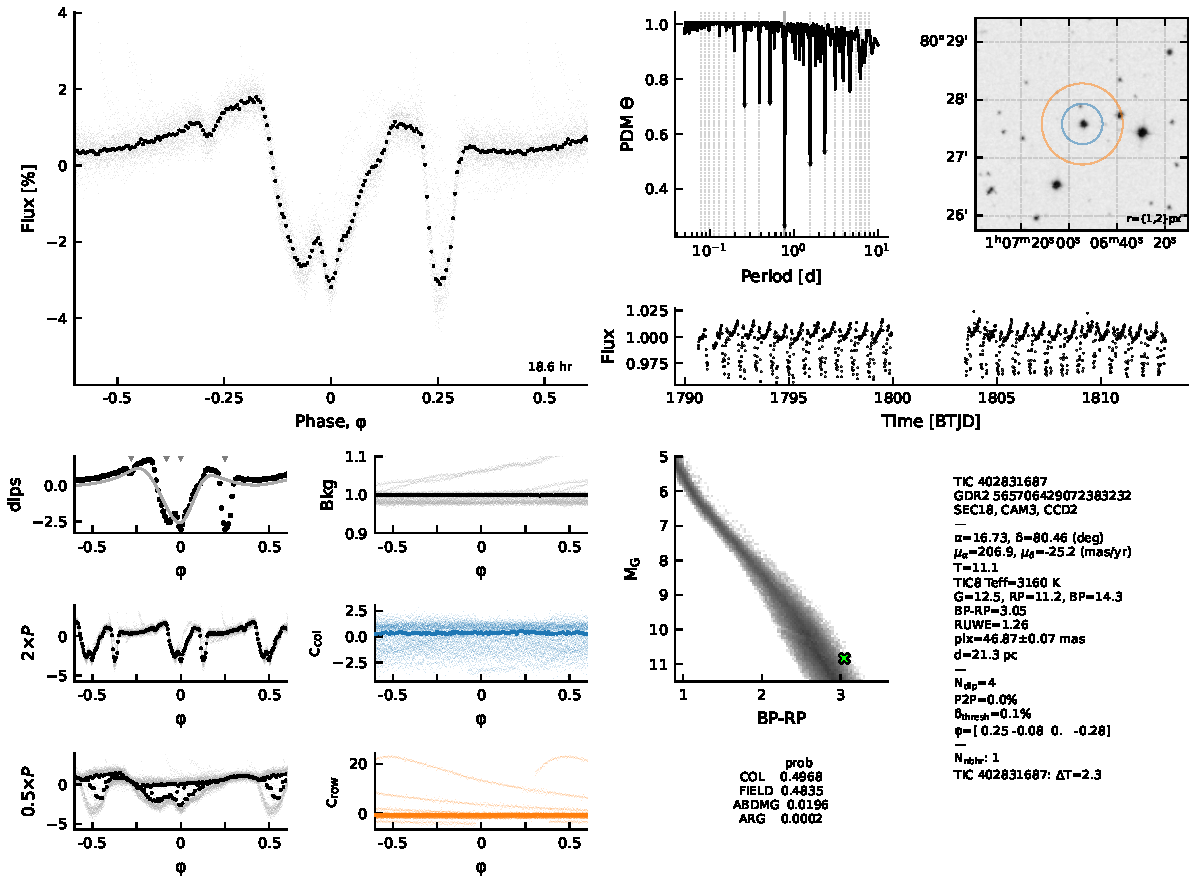
\includegraphics[width=0.96\textwidth]{402980664_S0018_120sec_cpvvetter.pdf}
		\vspace{-0.45cm}
		\caption{
      {\bf Validation plots used to label CQVs}.  The complete figure
      set of \ncpvsfound\ images is available online.
      Panels are as follows.
      {\it a)}: Phase-folded light curve; gray points are raw 2-minute
      data and black points are binned to 200 points per cycle.
      {\it b)}: Phase-dispersion minimization (PDM) periodogram.
      Dotted lines show up to the 10$^{\rm th}$ harmonic and
      subharmonic.
      {\it c)}: DSS finder chart, with 1- and 2-TESS pixel radius
      circles displayed for scale.
      {\it d)}: Cleaned light curve, binned to 20-minute cadence, in
      Barycentric TESS Julian Date (BTJD).
      {\it e)}: Phase-folded light curve, binned to 100 points per
      cycle.  The gray line denotes the automated spline-fit to the
      wrapped phase-folded light curve, and small gray triangles
      denote automatically identified local minima.
      {\it f)}: Phase-folded light curve at twice the peak period.
      {\it g)}: Phase-folded light curve at half the peak period.
      {\it h)}: Phase-folded time-series within the ``background''
      aperture defined in the SPOC light curves.
      {\it i)}: Phase-folded flux-weighted centroid in the column
      direction.
      {\it j)}: Phase-folded flux-weighted centroid in the row
      direction.
      {\it k)}: Gaia DR2 color--absolute magnitude diagram.     
      {\it l)}: Information from Gaia DR2, TIC8, and the automated
      dip-counting search pipeline.  ``Neighbors'', abbreviated
      ``nbhr'', are listed within apparent distances of 2 TESS pixels
      if $\Delta T$$<$2.5.
      {\it m)}: BANYAN-$\Sigma$ v1.2 association probabilities, calculated
      using positions, proper motions, and the parallax.
      }
		\label{fig:vet}
	\end{center}
\end{figure*}


\section{LP 12-502}

{\it The light curve}---
Figure~\ref{fig:lplc} shows an alternative view of the LP-502 light
curve from Figure~\ref{fig:lp}, 
split into ``time chunks'' wherever there was more than half a day of
missing data in the TESS light curve.
We binned the light curve to 15-minute intervals for visual clarity,
and required at least one (120-second cadence) flux measurement per
bin.
Points more than 2.5$\sigma$ above the median are drawn in gray, also
for visual clarity.
Missing data are not drawn (a common plotting error when ``drawing''
light curves, rather than showing a scatter plot).

{\it State switches}---
Figure~\ref{fig:lpzoom} shows an alternative view of cycles 1233-1247.

\begin{figure*}[!t]
	\begin{center}
		\centering
		\includegraphics[width=0.96\textwidth]{tic4029_segments.pdf}
		\vspace{-0.2cm}
		\caption{
      {\bf LP 12-502 light curve}, split into time chunks.
		}
		\label{fig:lplc}
	\end{center}
\end{figure*}


\begin{figure*}[!t]
	\begin{center}
    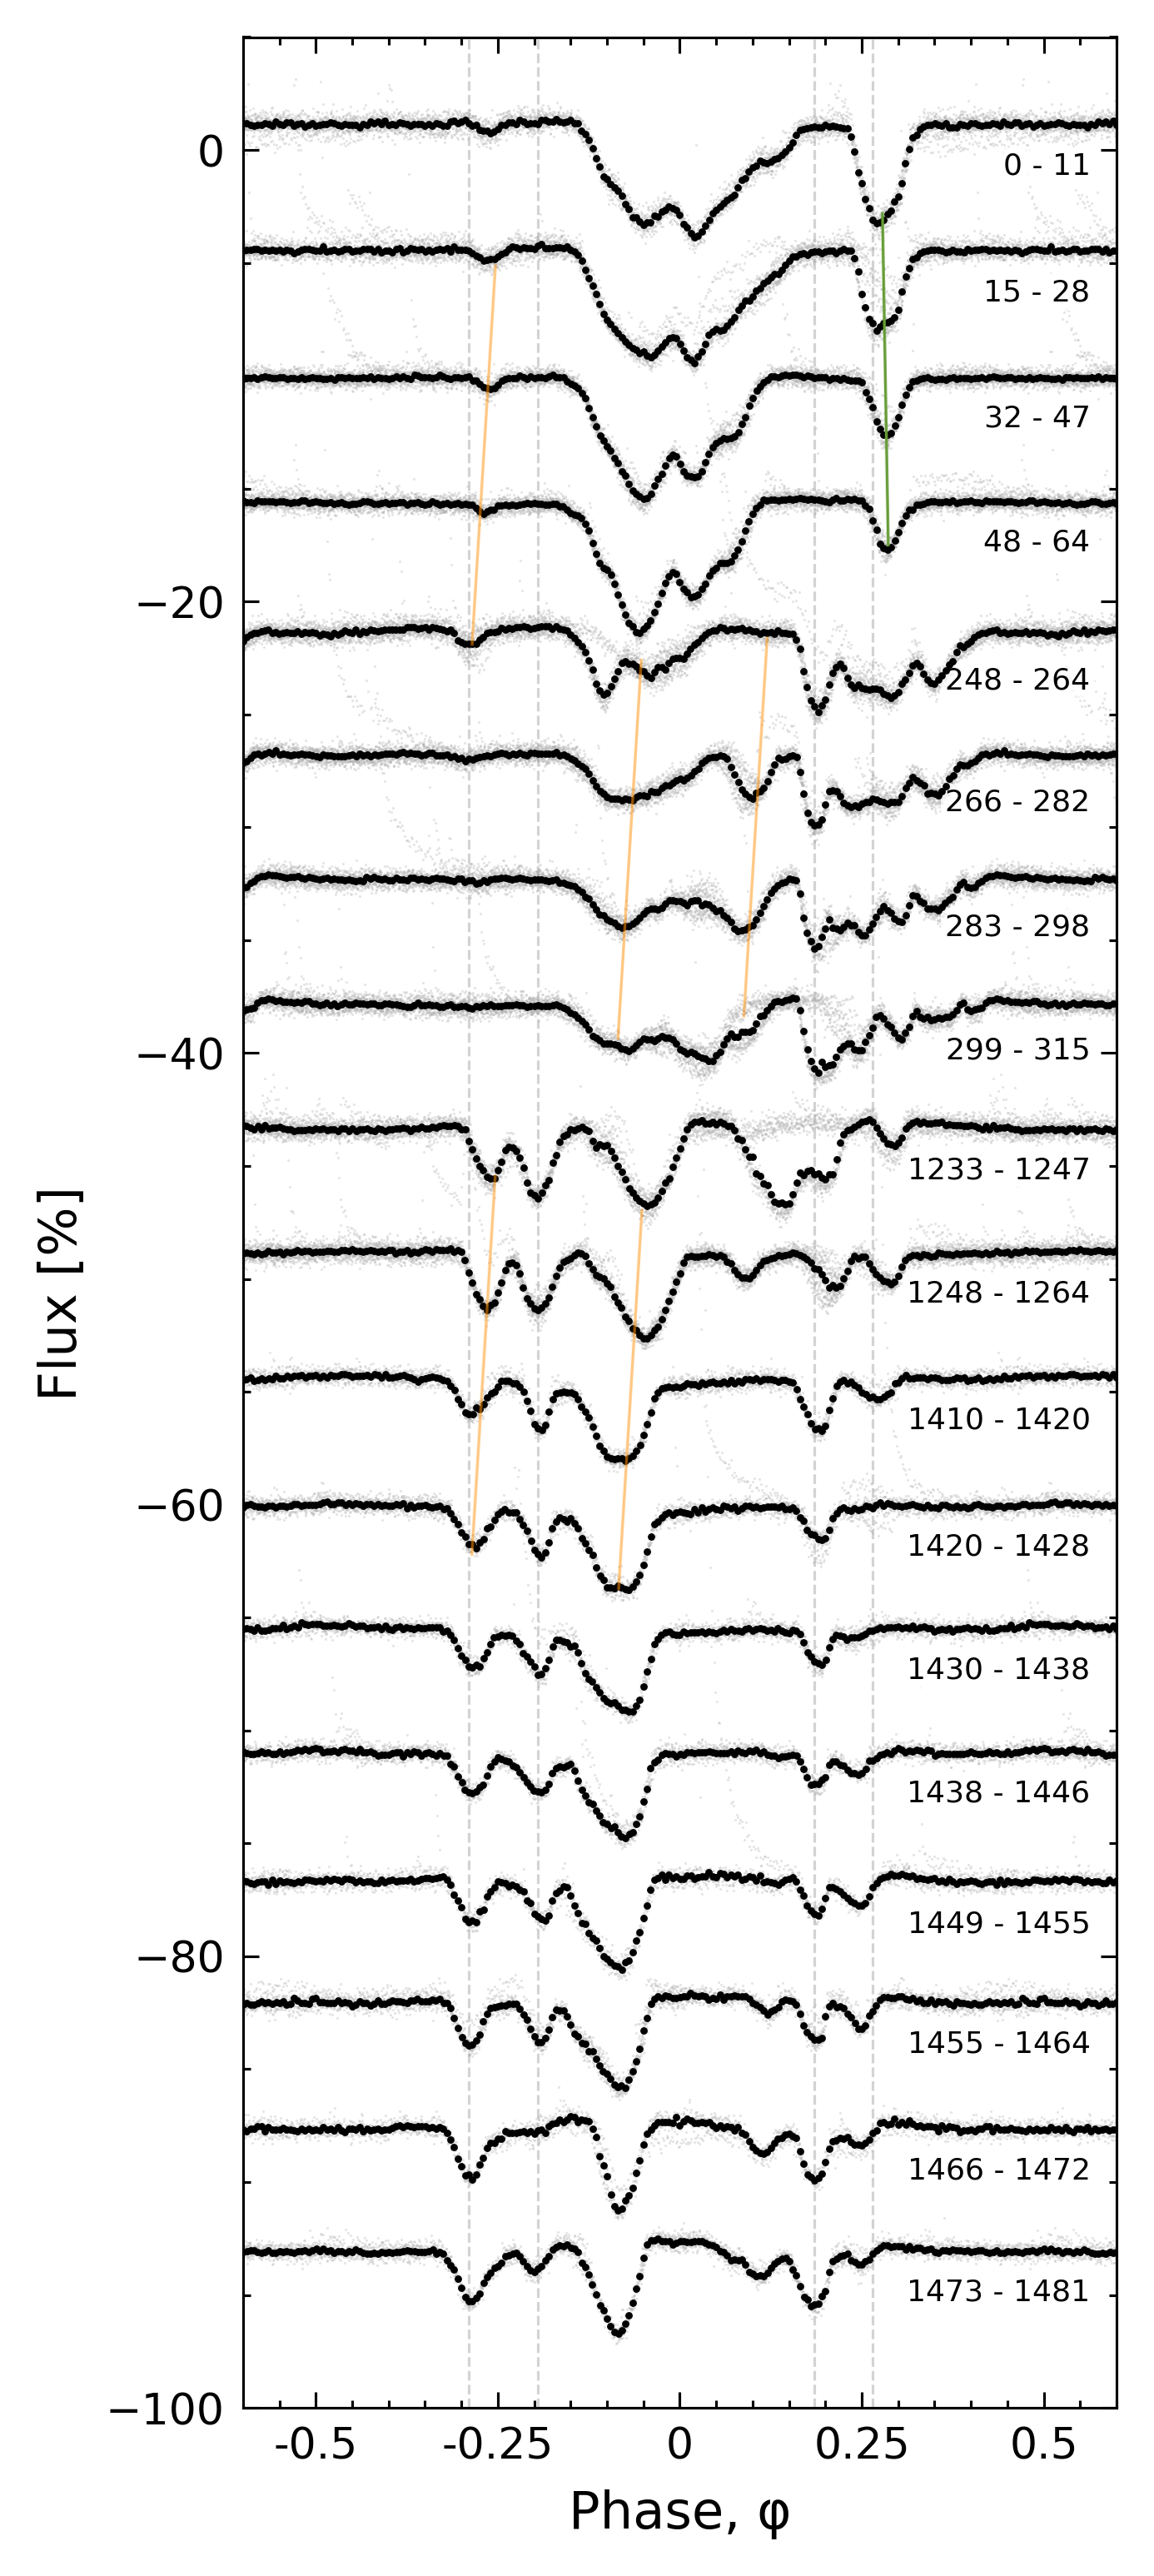
\includegraphics[width=0.45\textwidth]{ANNOTATED_resid_TIC_402980664_P18.5611_2min_phase_timegroups.png}
    	\end{center}
    \vspace{-0.4cm}
		\caption{
	      {\bf Alternative view of the evolution of LP 12-502}
	      (Figure~\ref{fig:lp}), arranged to emphasize changes in transit
	      times.  There are 200 binned black points per cycle; a two-harmonic
	      sinusoid has been subtracted over specific chunks in time ({\bf see text}).
	      Vertical gray lines are underplotted to help guide the eye to instances
	      in which preferred dip phases synchronize over long baselines.
	      The orange and green lines guide the eye to where dips
	      appear to change the positions of their local minima.
		}
		\label{fig:lp2}
\end{figure*}


\begin{figure*}[!t]
	\begin{center}
		\subfloat{
			\includegraphics[width=0.43\textwidth]{TIC402980664_river_gist_stern_0_64_manual_20230617_mask_v0_nterms2_vmin-0.04000_vmax0.01000.png}
			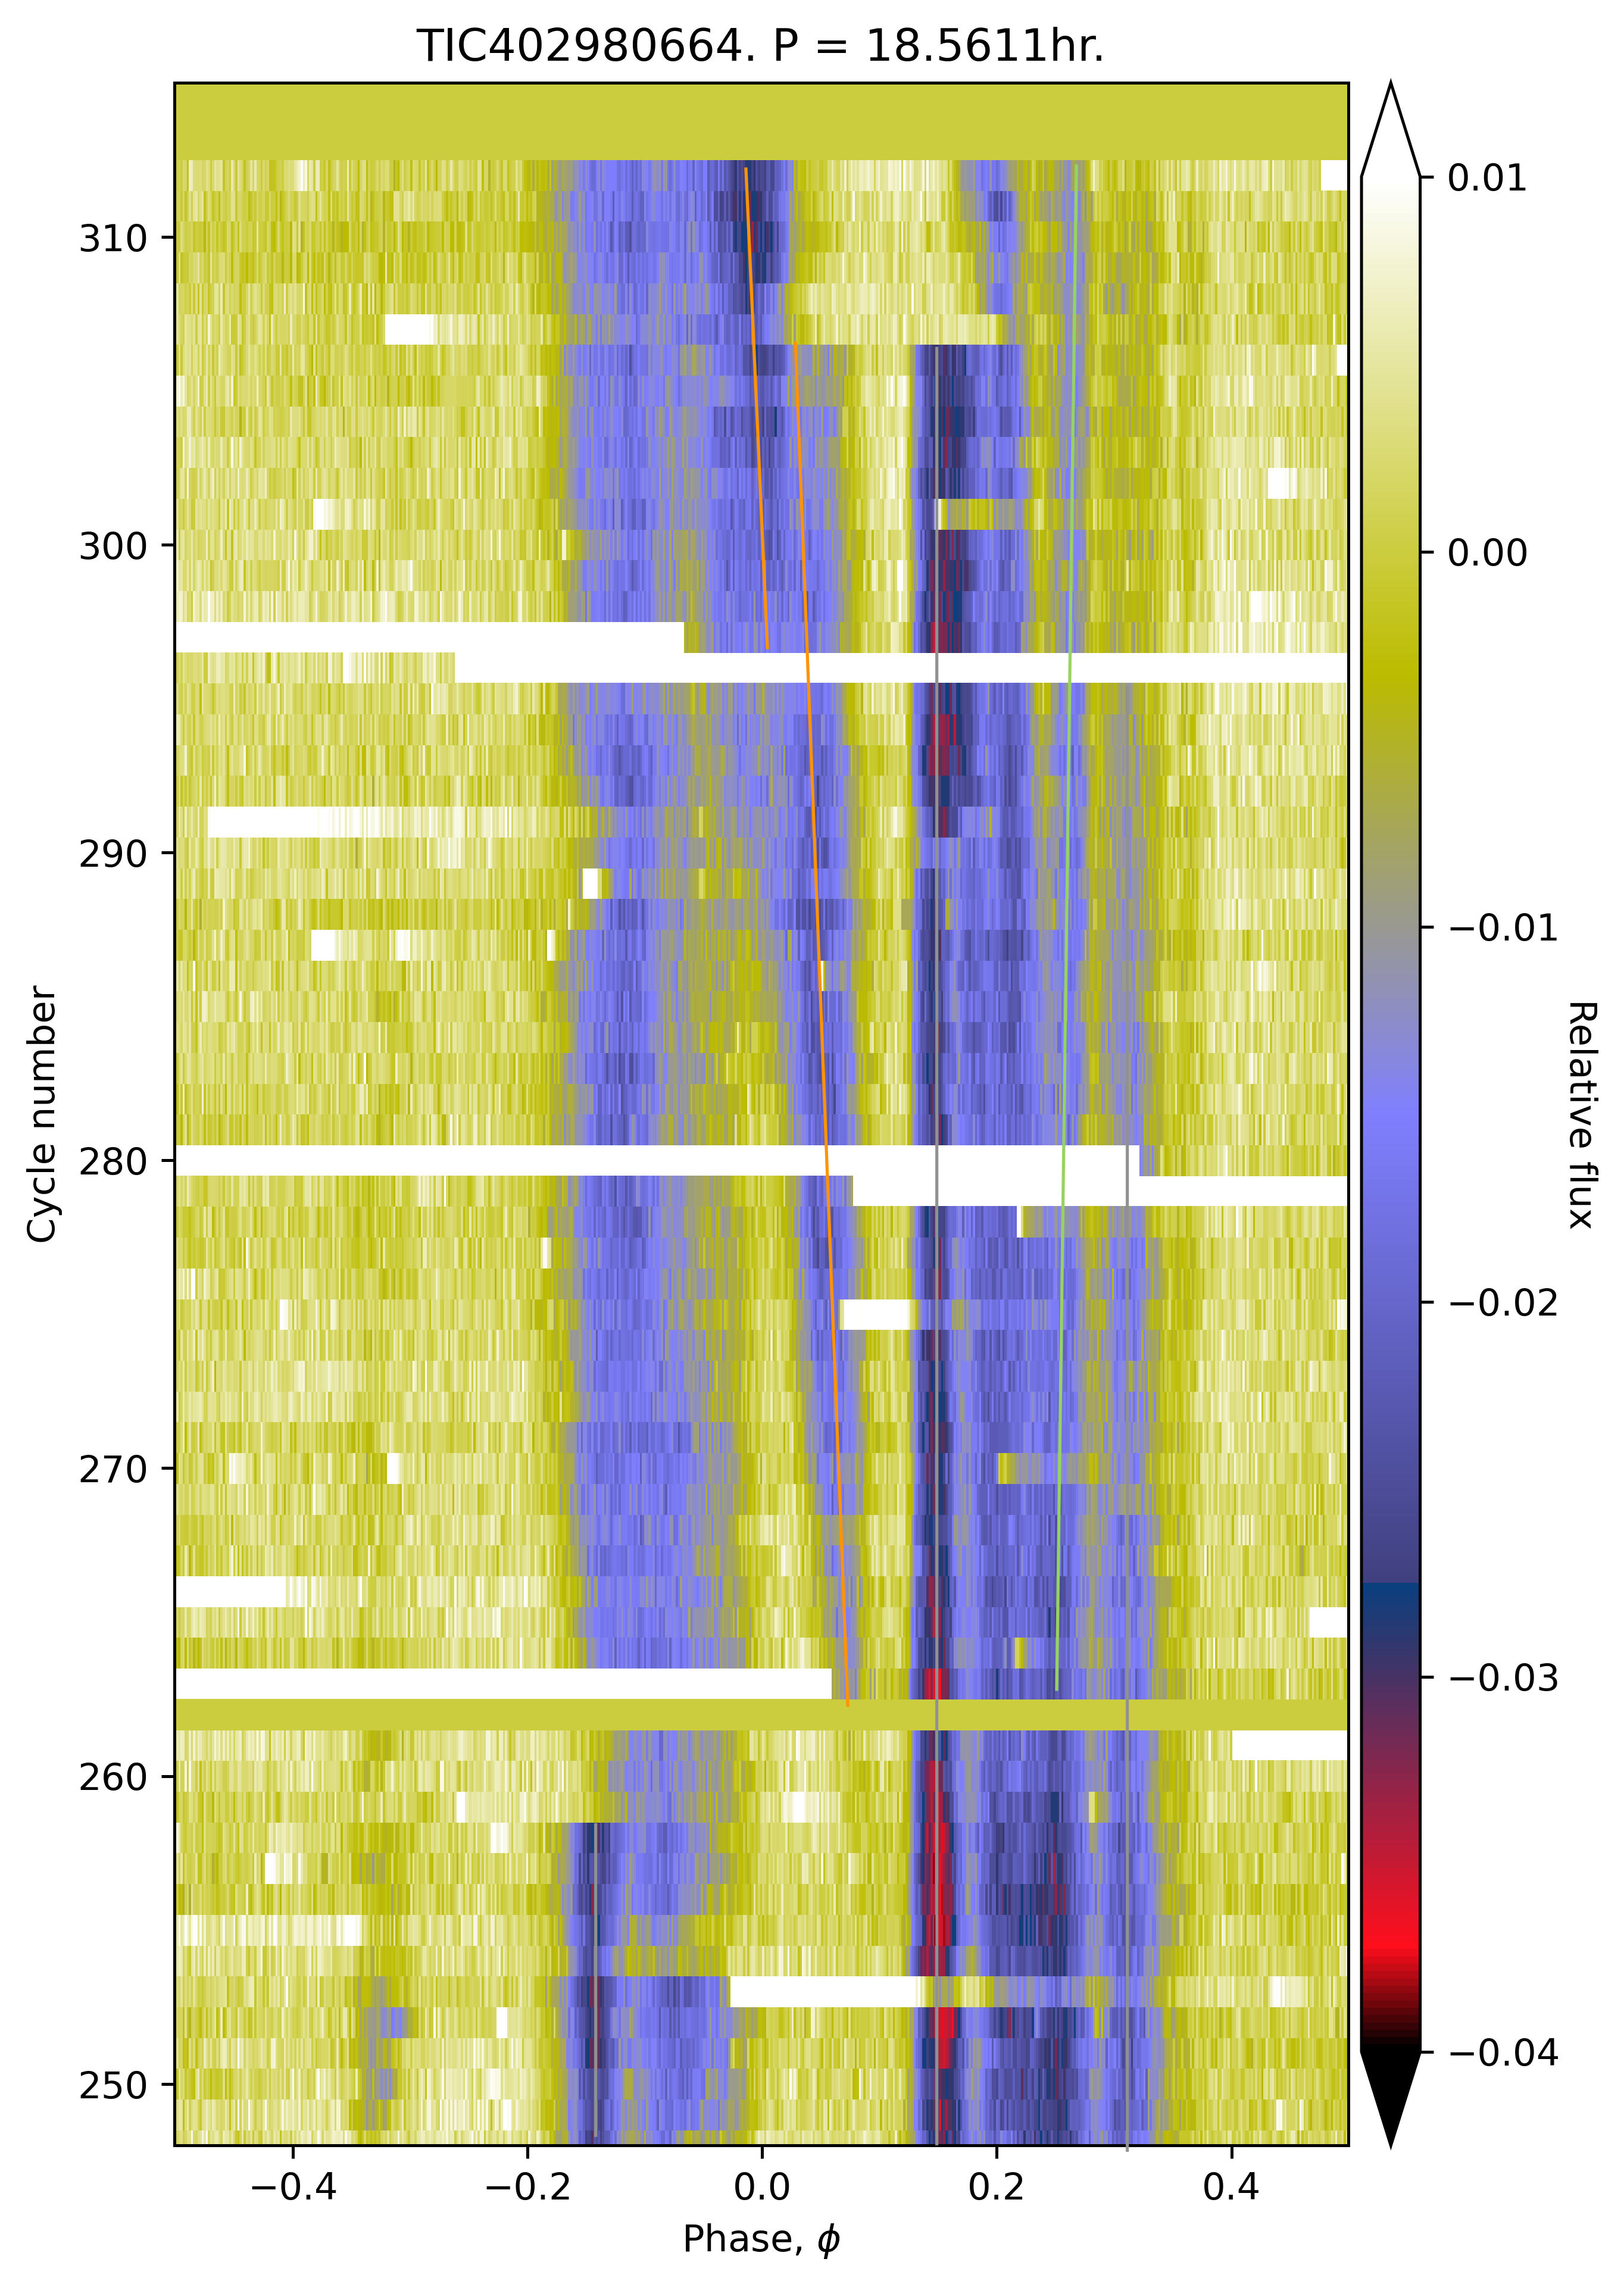
\includegraphics[width=0.43\textwidth]{ANNOTATED_TIC402980664_river_gist_stern_248_315_manual_20230617_mask_v0_nterms2_vmin-0.04000_vmax0.01000.png}
		}
	\vspace{-0.1cm}
			\subfloat{
		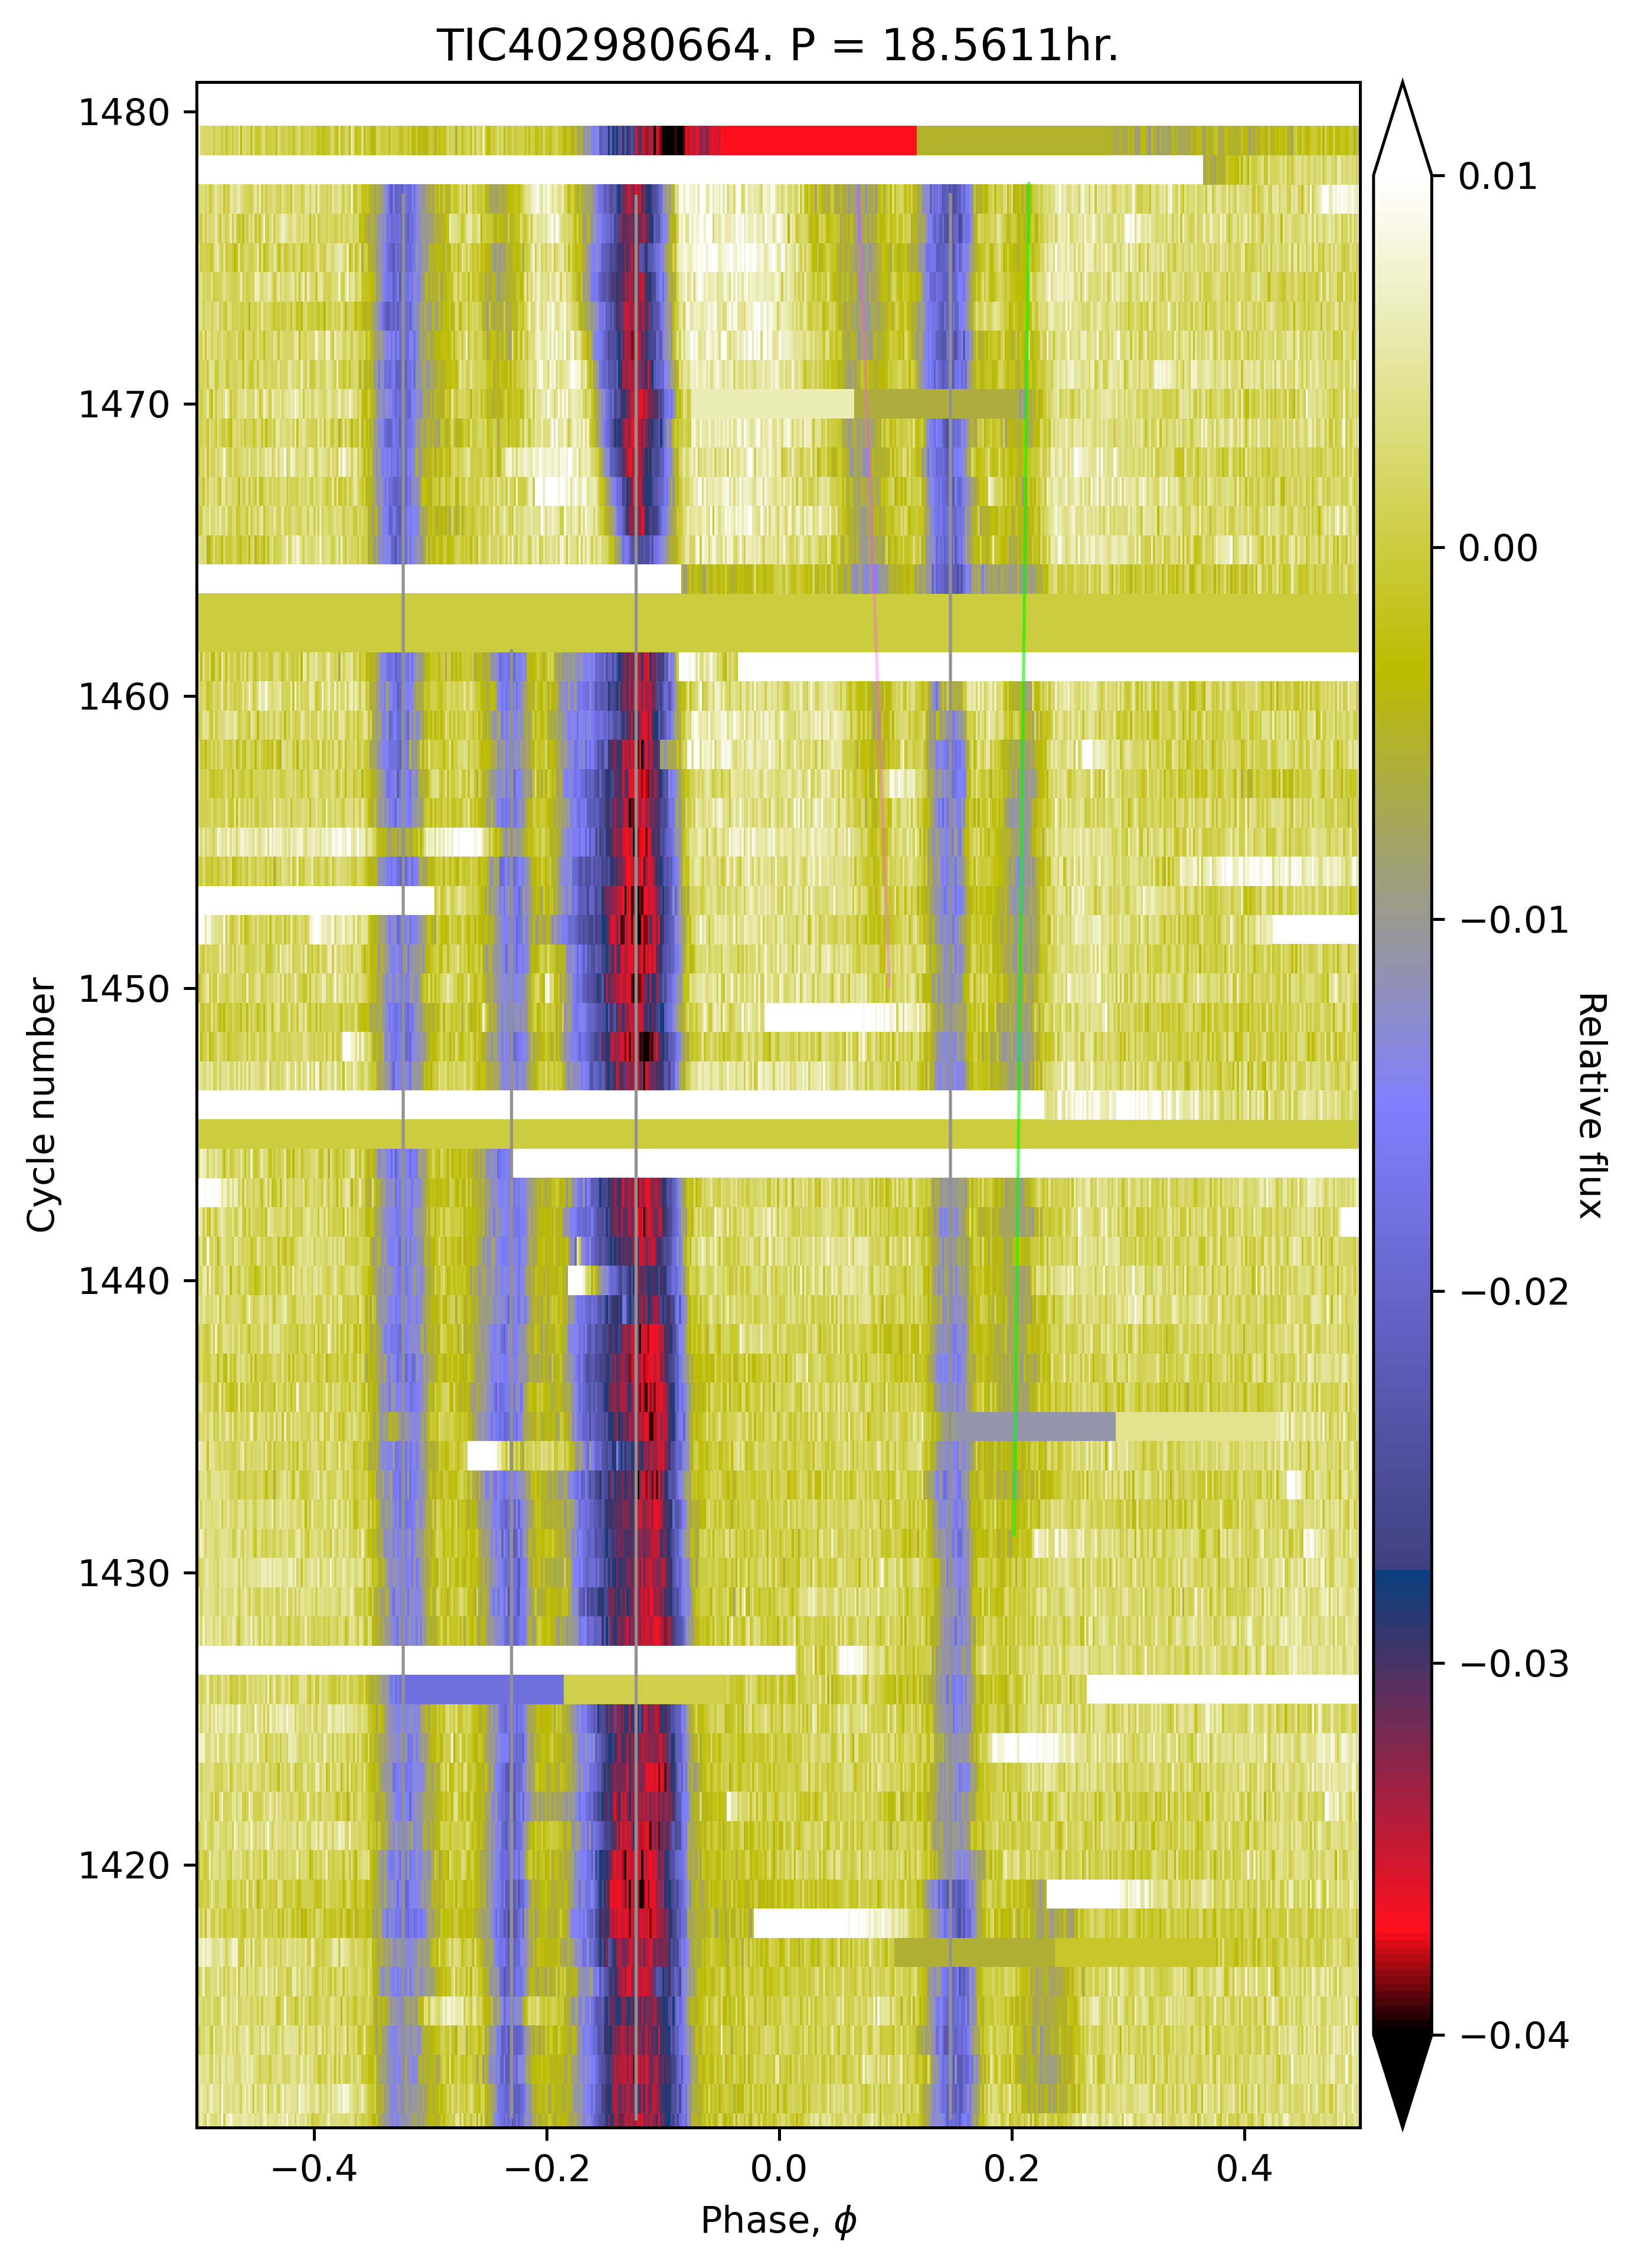
\includegraphics[width=0.43\textwidth]{ANNOTATED_TIC402980664_river_gist_stern_1411_1481_manual_20230617_mask_v0_nterms2_vmin-0.04000_vmax0.01000.png}
				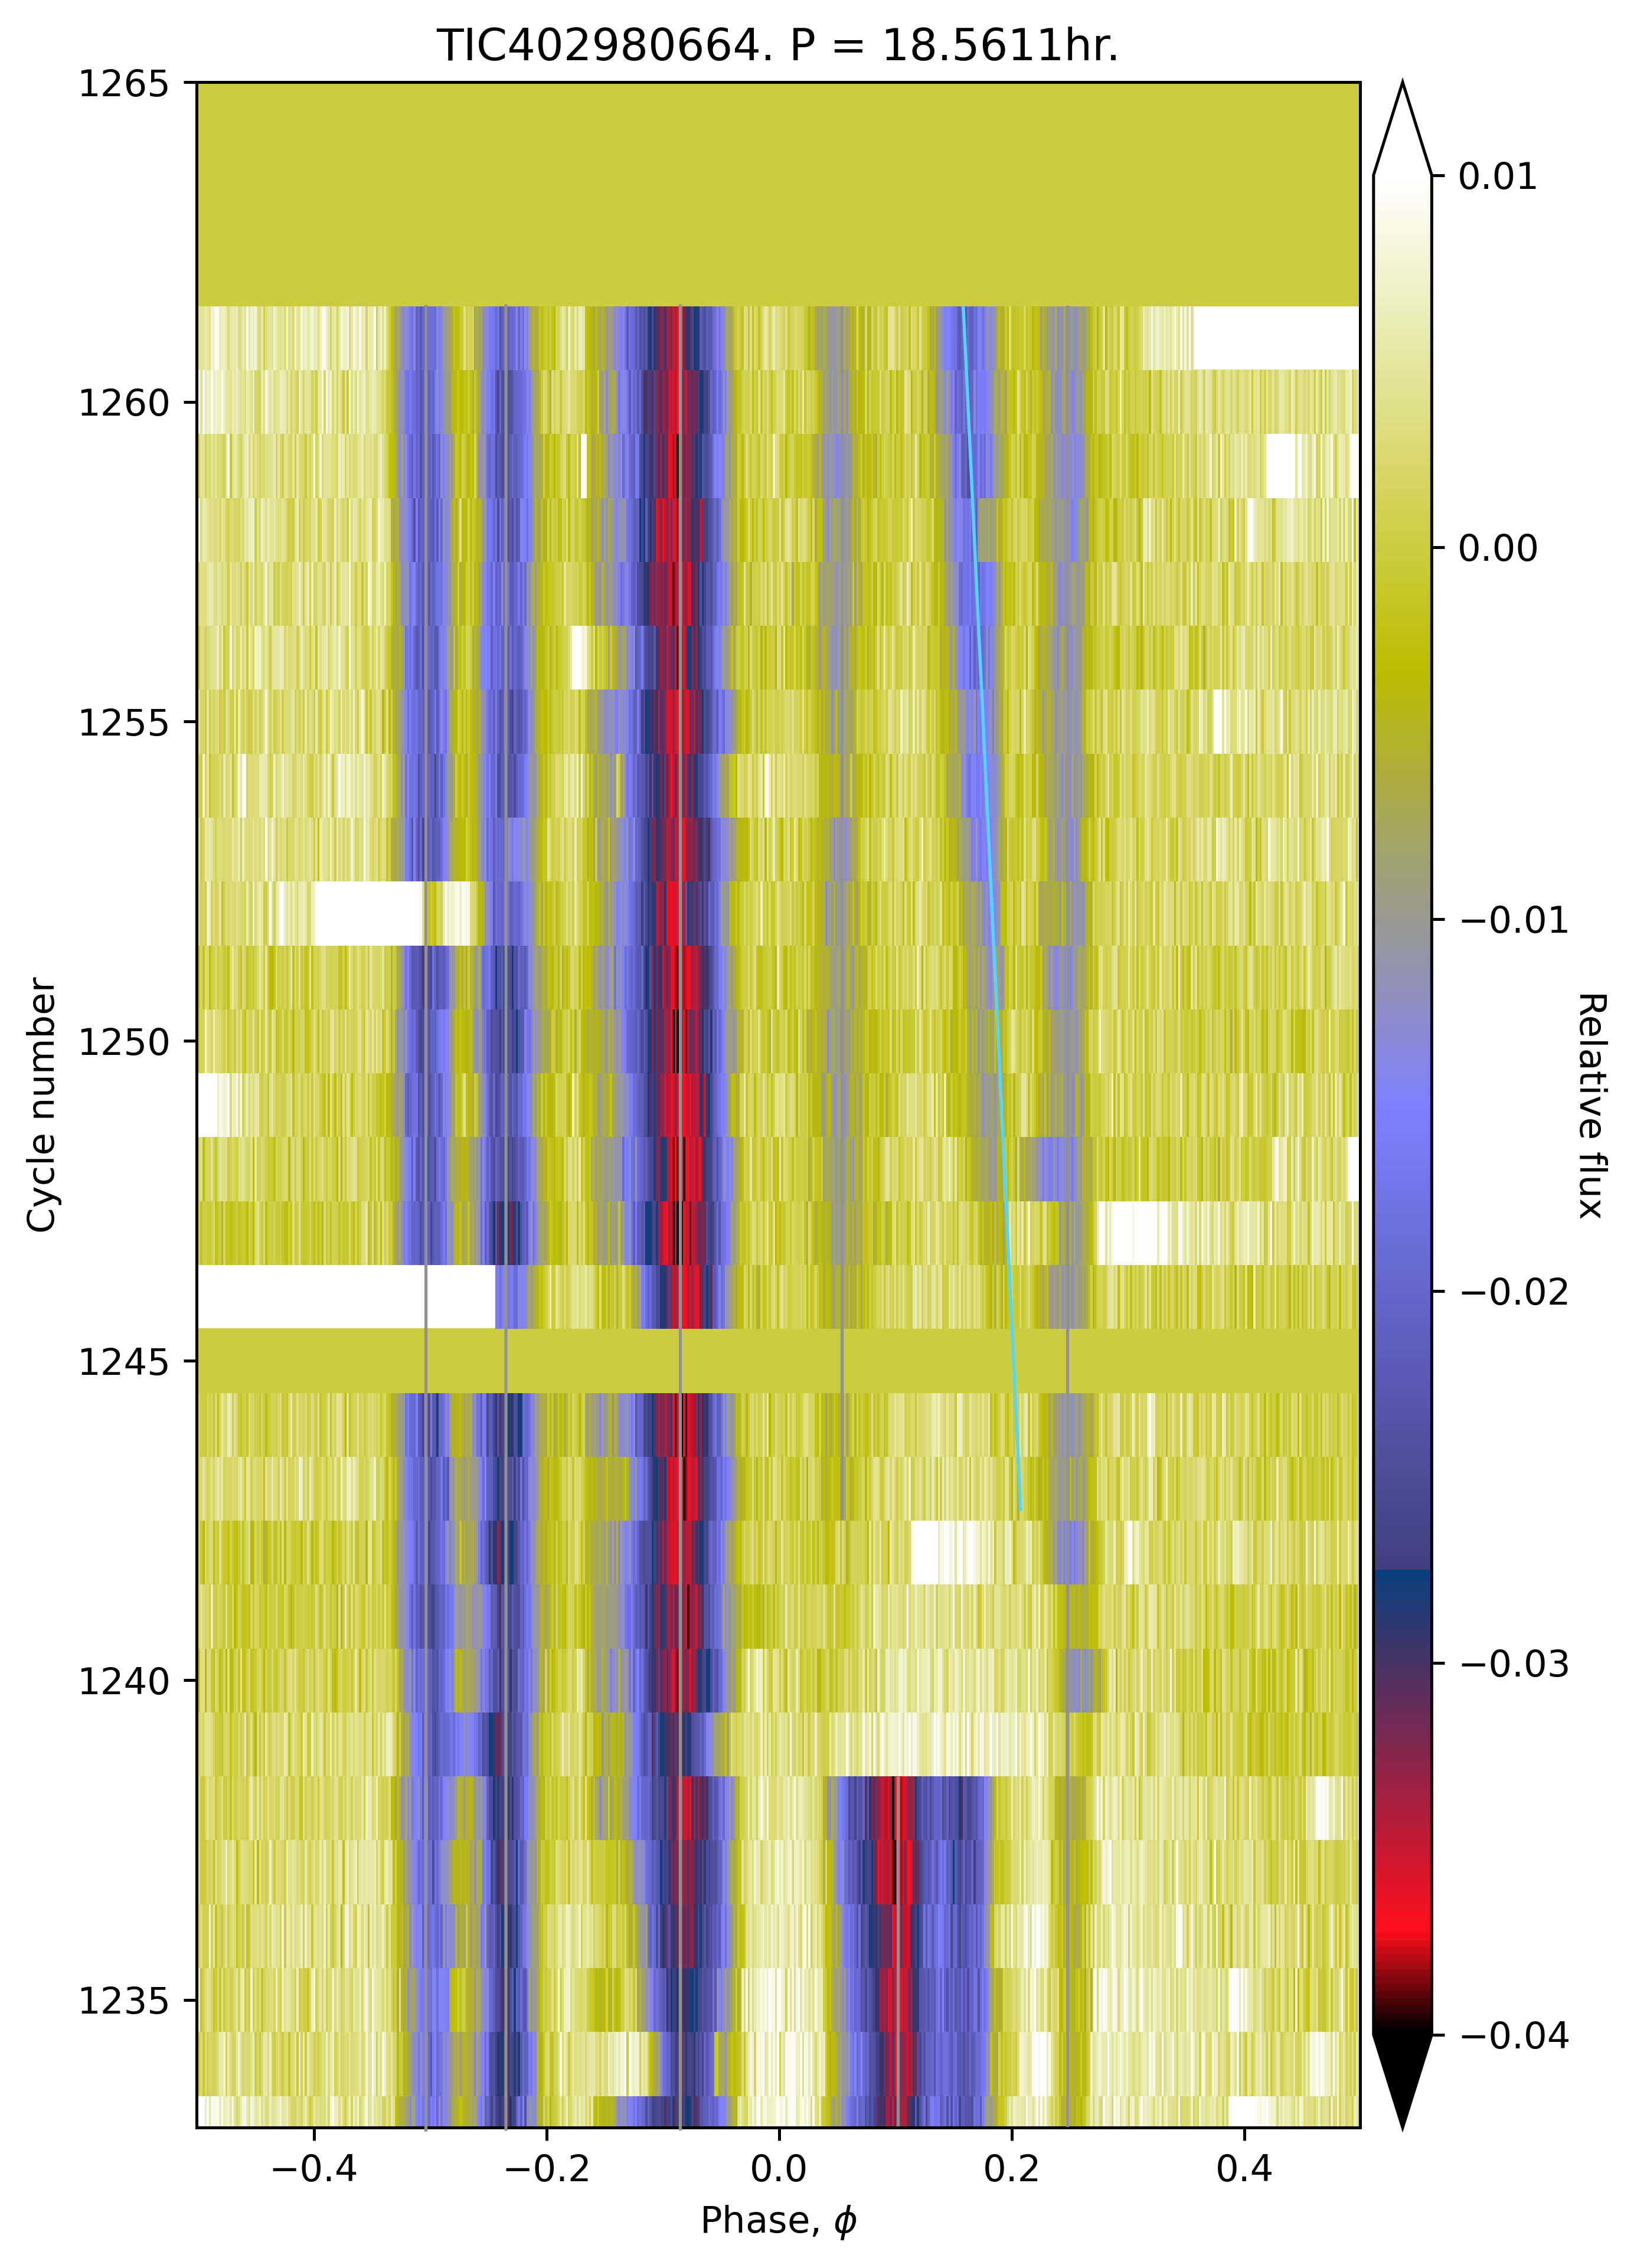
\includegraphics[width=0.43\textwidth]{ANNOTATED_TIC402980664_river_gist_stern_1233_1265_manual_20230617_mask_v0_nterms2_vmin-0.04000_vmax0.01000.png}
	}
	\end{center}
	\caption{
    {\bf River plots of LP 12-502}, showing (clockwise from top-left)
    Sectors 18-19, 25-26, 53, and 58-59.  A two-harmonic sinusoid has
    been subtracted over specific chunks in time ({\bf see text}).
    For Sectors 25-26 (cycles 248-315), three periods are overplotted:
    $P$=18.5611\,hr (gray vertical line); 18.5404\,hr (orange); 18.5683\,hr (green).
    For Sector 53, gray is identical, while cyan is 18.5145\,hr.
    For Sectors 58-59, the magenta line is 18.5473\,hr, and the green
    line is 18.5672\,hr.
	}
	\label{fig:lpriver0}
\end{figure*}


\begin{figure*}[!t]
	\begin{center}
		\centering
		\includegraphics[width=0.96\textwidth]{TIC4029_zoom.png}
		\vspace{-0.45cm}
		\caption{
			{\bf LP 12-502 cycles 1233-1247}, showing the most dramatic state
			change observed over the three year baseline.
		}
		\label{fig:lpzoom}
	\end{center}
\end{figure*}


\section{No additional power at 20~second cadence}

Going from K2 to TESS, an important discovery was that the CQV shapes
can significantly evolve, since the stars can vary over timescales of just a few minutes.
We observed a set of CQVs between 2020 and 2021 using the TESS 20-second
cadence mode (TESS DDT029).
{\bf todo: list the stars.  todo: examine the 2min vs 20sec periodograms, and summarize in a few
sentences whether any difference is there.}






\clearpage
\listofchanges


\end{document}
